\chapter{Mejoras a WebSim}
\label{chap:mejoras}
Una vez presentado el contexto, objetivos y herramientas empleadas, en este capitulo se detallan todas las mejoras realizadas del simulador \textit{WebSim} y cómo se han llevado a cabo. 

\section{Drone}
Uno de los objetivos principales del TFG era ampliar el soporte para otros robots y escenarios en \textit{WebSim}. Se ha comenzado dando soporte a drones debido a las diferencias con el \textit{piBot} del que ya disponía soporte. 
Para ello hay que extender el \textit{software} existente de la plataforma.
\subsection{Drivers}
Una de las principales diferencias es el movimiento vertical, tanto para darle velocidad al \textit{drone} como para actualizar la posición. 
Se han creado las siguiente funciones para ello:
\begin{itemize}
    \item \textit{\textbf{setL()}}: Método que permite ordenar velocidad vertical al \textit{robot}. 
    
    \item \textit{\textbf{getV()}}: Método que devuelve la velocidad vertical del \textit{robot}.
    
    \item \textit{\textit{\textbf{despegar}}}: Método que da velocidad vertical al \textit{robot} hasta alcanzar cierta altura.
    
    \item \textit{\textbf{aterrizar}}: Método que da velocidad vertical negativa al \textit{robot} hasta que alcance el suelo. 
\end{itemize}

Además, se ha editado la función \textit{move} para que acepte 3 parámetros (añadiendo velocidad vertical como nuevo parámetro) y se ha extendido la función \textit{updatePosition()} para poder actualizar el eje Y en la escena de \textit{WebSim}.

\begin{lstlisting}[language=javascript, caption=Función para actualizar la posición del robot en el escenario]
    updatePosition(rotation, velocity, robotPos){
      let x = velocity.x/10 * Math.cos(rotation.y * Math.PI/180);
      let z = velocity.x/10 * Math.sin(-rotation.y * Math.PI/180);
      let y = (velocity.y/10);
      robotPos.x += x;
      robotPos.z += z;
      robotPos.y += y;
      return robotPos;
    }
\end{lstlisting}

En la tabla \ref{tab:tablaMotores2} se explican todas las funciones del \textit{HAL API} que extienden la plataforma para dar soporte al \textit{drone}.

\begin{table}[H]
  \begin{center}
    \caption{Métodos (HAL API) de los actuadores implementados para el drone.}
    \vspace{0.5cm}
    \label{tab:tablaMotores2}
    \begin{tabular}{|c|c|} 
    \hline
      \textbf{Método} & \textbf{Descripción}\\
      \hline
.setL(integer) & \begin{tabular}[c]{@{}c@{}}Mueve hacia arriba o hacia abajo el robot.\\\end{tabular} \\ \hline
.getL() & \begin{tabular}[c]{@{}c@{}}Devuelve la velocidad vertical del robot.\\\end{tabular} \\ \hline
.move(integer, integer, integer) & \begin{tabular}[c]{@{}c@{}}Mueve el robot hacia delante/atrás,\\ arriba/abajo y gira al mismo tiempo.\\ \end{tabular} \\ \hline
.despegar() & \begin{tabular}[c]{@{}c@{}}Comanda velocidad vertical al robot hasta que \\ alcanza una determinada altura.\\ \end{tabular} \\ \hline
.aterrizar() & \begin{tabular}[c]{@{}c@{}}Comanda velocidad vertical negativa al robot hasta que \\ alcanza el suelo.\\ \end{tabular} \\ \hline
    \end{tabular}
  \end{center}
\end{table}

Uno de los principales problemas encontrados es que el motor de físicas de \textit{A-Frame} no simula correctamente la posición de robot al otorgarle velocidad vertical y hace que el robot ``rebote'' sobre el escenario. Esto es debido a que el escenario tiene un atributo llamado gravedad que se aplica cada pocos milisegundos y entra en conflicto con la función \textit{updatePosition}. Se ha solucionado cambiando su valor haciendo que el escenario carezca de gravedad cuando se simula el \textit{drone}. Además, se han realizado una serie de pruebas para comprobar el comportamiento del \textit{drone}. \newline

El coste computacional aumenta al otorgarle gravedad al escenario porque hay que aumentar las iteraciones en las que el motor de físicas de \textit{A-Frame} actúa. De este manera, a más iteraciones más realista es la simulación de la gravedad, pero mayor es el coste computacional.

Los resultados obtenidos se pueden observar en la tabla \ref{tab:tablaGravedad}.

\begin{table}[H]
\caption{Pruebas de valores de gravedad e iteraciones}
\centering
\label{tab:tablaGravedad}
\begin{tabular}{|c|c|c|c|c|c|}
\hline
\multicolumn{1}{|l|}{\textbf{Gravedad}} & \multicolumn{1}{l|}{\textbf{Iteraciones}} & \multicolumn{1}{l|}{\textbf{Mín. IPS}} & \multicolumn{1}{l|}{\textbf{Máx. IPS}} & \multicolumn{1}{l|}{\textbf{Media IPS}} & \multicolumn{1}{l|}{\textbf{Coste gráfico}} \\ \hline
-4 & 30000 & 17 & 60 & 47 & 32.95\% \\ \hline
-4 & 50000 & 3 & 60 & 50 & 38.82\% \\ \hline
-2.5 & 1000000 & 3 & 60 & 51 & 41.72\% \\ \hline
-3.5 & 1000000 & 33 & 60 & 50 & 41.5\% \\ \hline
\end{tabular}
\end{table}

El mejor resultado se ha obtenido fijando la gravedad a -3.5 y las iteraciones a 1000000, de esta manera existe gravedad en el escenario y no supone un coste computacional demasiado grande. 

\subsection{Bloques Scratch}

Una vez implementado el código \textit{JavaScript} para el soporte del drone, es necesario crear los bloques con \textit{Blockly} para poder añadir sus funcionalidad en el editor de \textit{Scratch}. 

Para ello, se han creado 4 bloques con las funciones anteriormente explicadas: 
\begin{itemize}
    \item Velocidad ascenso: Comanda la velocidad ascendente del bloque que se le adjunte. 
    \begin{figure}[H]
        \centering
        
\includegraphics[width=0.3\textwidth]{img/ascensionBlockly.png}
        \caption{Bloque de velocidad de ascenso} \label{fig:ascension}
    \end{figure}
    
    \item Velocidad descenso: Comanda al robot la velocidad descendente del bloque que se le adjunte. 
    \begin{figure}[H]
        \centering
        
\includegraphics[width=0.3\textwidth]{img/descensoBlockly.png}
        \caption{Bloque de velocidad de descenso} \label{fig:descenso}
    \end{figure}
    \item Aterrizar: Comanda velocidad vertical al \textit{drone} hasta que alcance cierta altitud. Mantendrá esa posición hasta recibir una nueva orden.
    \begin{figure}[H]
        \centering
        
\includegraphics[width=0.2\textwidth]{img/aterrizarBlockly.png}
        \caption{Bloque de aterrizaje} \label{fig:aterrizaje}
    \end{figure}
    \item Despegar: Comanda velocidad vertical negativa al \textit{drone} hasta que alcance el suelo. 
        \begin{figure}[H]
            \centering
            
\includegraphics[width=0.2\textwidth]{img/despegarBlockly.png}
            \caption{Bloque de despegue} \label{fig:despegar}
        \end{figure}
\end{itemize}

Para que los bloques aparezcan en el editor de \textit{Scratch} es necesario importarlos e inicializarlos en el fichero que lo configura. Se pueden ver los bloques traducidos a inglés e implementados en el espacio de trabajo en la figura {\ref{fig:newblocks}}.

        \begin{figure}[H]
            \centering
            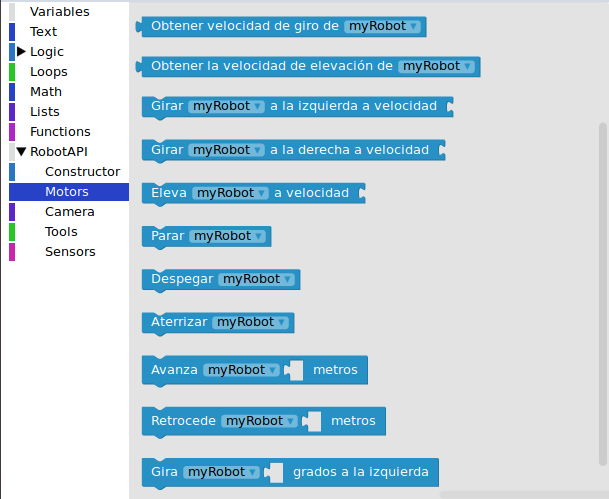
\includegraphics[width=0.65\textwidth]{img/kibotics_newblocks.png}
            \caption{Espacio de trabajo de \textit{Scratch} con los bloques del drone incorporados} 
            \label{fig:newblocks}
        \end{figure}

\subsection{Modelo 3D}

Para simular el robot en el entorno de \textit{A-Frame} es necesario realizar un modelo tridimensional. Para ello se ha buscado un modelo en una librería\footnote{\url{https://sketchfab.com/}} y se ha editado en \textit{Blender} (figura \ref{fig:droneBlender}) para que se ajuste a los requisitos del entorno. Las modificaciones que se han realizado al modelo son: 
\begin{itemize}
    \item Reducción de polinomios  para que no se ralentice la carga del mundo.
    \item Rotación del modelo para que encaje con la orientación que disponía el anterior robot. Es decir, que el robot tenga su parte frontal mirando hacia el eje X positivo para que al comandarle velocidad lineal se desplace hacia delante.
    \item Modificación de la luz para adaptarla al escenario de \textit{WebSim}. 
    
    \item Elaborar una animación a las hélices para darle un aspecto más realista. Esta animación se activa vía \textit{software} cuando el drone despega del suelo\footnote{\url{https://www.youtube.com/watch?v=XjQNhNCkOJA}}.
\end{itemize}

 \begin{figure}
    \centering
    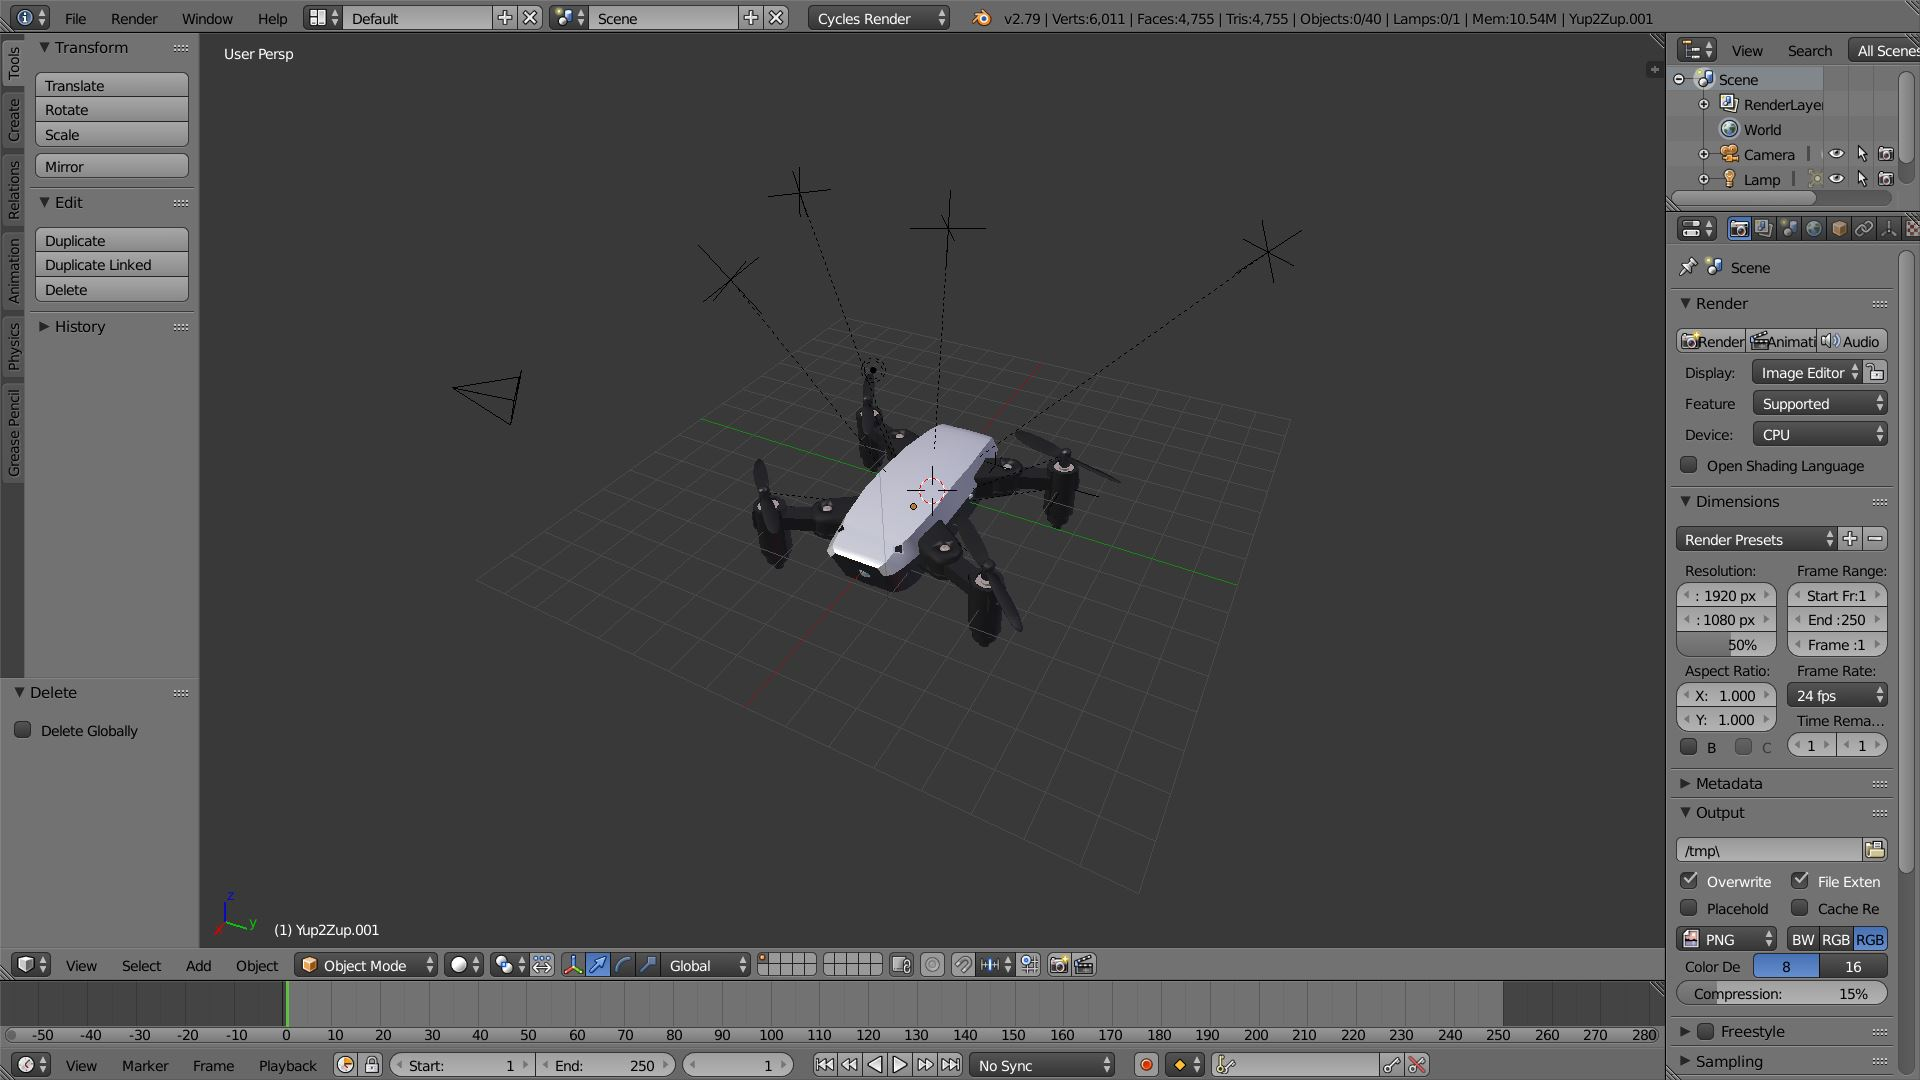
\includegraphics[scale=0.3]{img/droneBlender.jpg}
    \caption{Drone en Blender} \label{fig:droneBlender}
\end{figure}

El drone implementado en el entorno de \textit{Websim} se puede ver en la figura \ref{fig:escenarioDrone}.
   \begin{figure}[H]
    \centering
    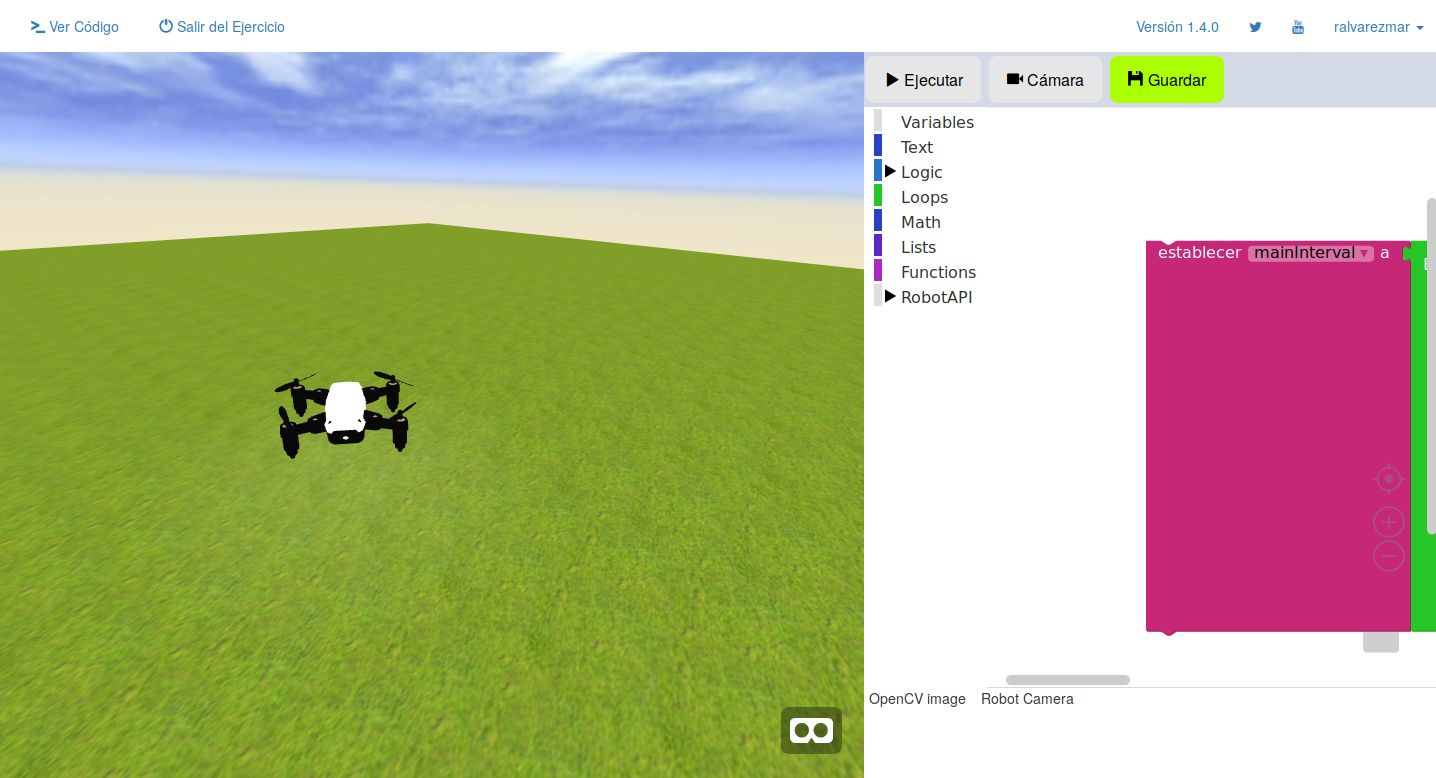
\includegraphics[scale=0.3]{img/websimDrone.png}
    \caption{Escenario de WebSim con drone integrado} \label{fig:escenarioDrone}
    \end{figure}


\section{Escenarios}

Se han incorporado nuevos escenarios a \textit{WebSim} que dan la posibilidad de realizar nuevos ejercicios y  mejorar los ya disponibles. En esta sección se explicarán los escenarios con un solo robot y se hará mención a lo que tienen con dos robots, que se explicarán en profundidad más adelante.

\subsection{Sigue-líneas visión}
    Se ha mejorado el escenario cambiando la textura del suelo a una creada con la trazada del circuito de Interlagos. Se ha realizado con un programa de diseño gráfico y, debido a su peso, se ha reducido posteriormente su tamaño para aliviar los tiempos de carga. 
    
    \begin{figure}[H]
    \centering
    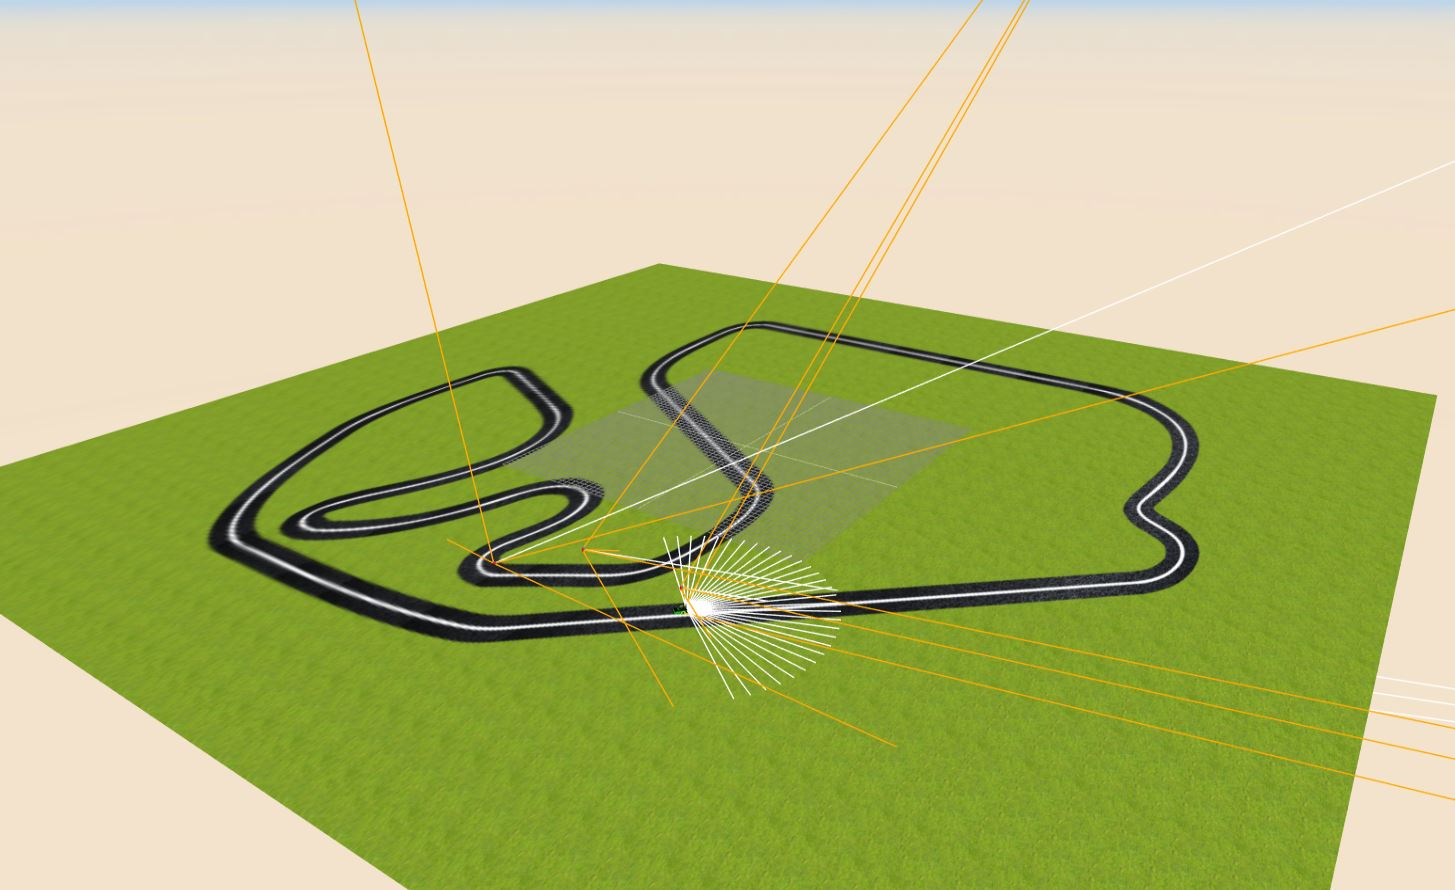
\includegraphics[scale=0.4]{img/pibot_vision.JPG}
    \caption{Escenario para el ejercicio \textit{piBot} sigue-líneas con cámara} \label{fig:siguelineavision}
    \end{figure}
    
\subsection{Sigue-líneas infrarrojos}
    Con un recorrido similar a sigue-líneas visión, pero con fondo blanco y recorrido negro para facilitar la implementación de código al robot real y que no haya que realizar modificaciones. Para que funcionara correctamente ha sido necesario añadir el color blanco a \textit{undestandedColors} para realizar el filtro y poder pasar ``\textit{white}'' como atributo a la función \textit{getObjectColor()}.
    
    \begin{figure}[H]
    \centering
    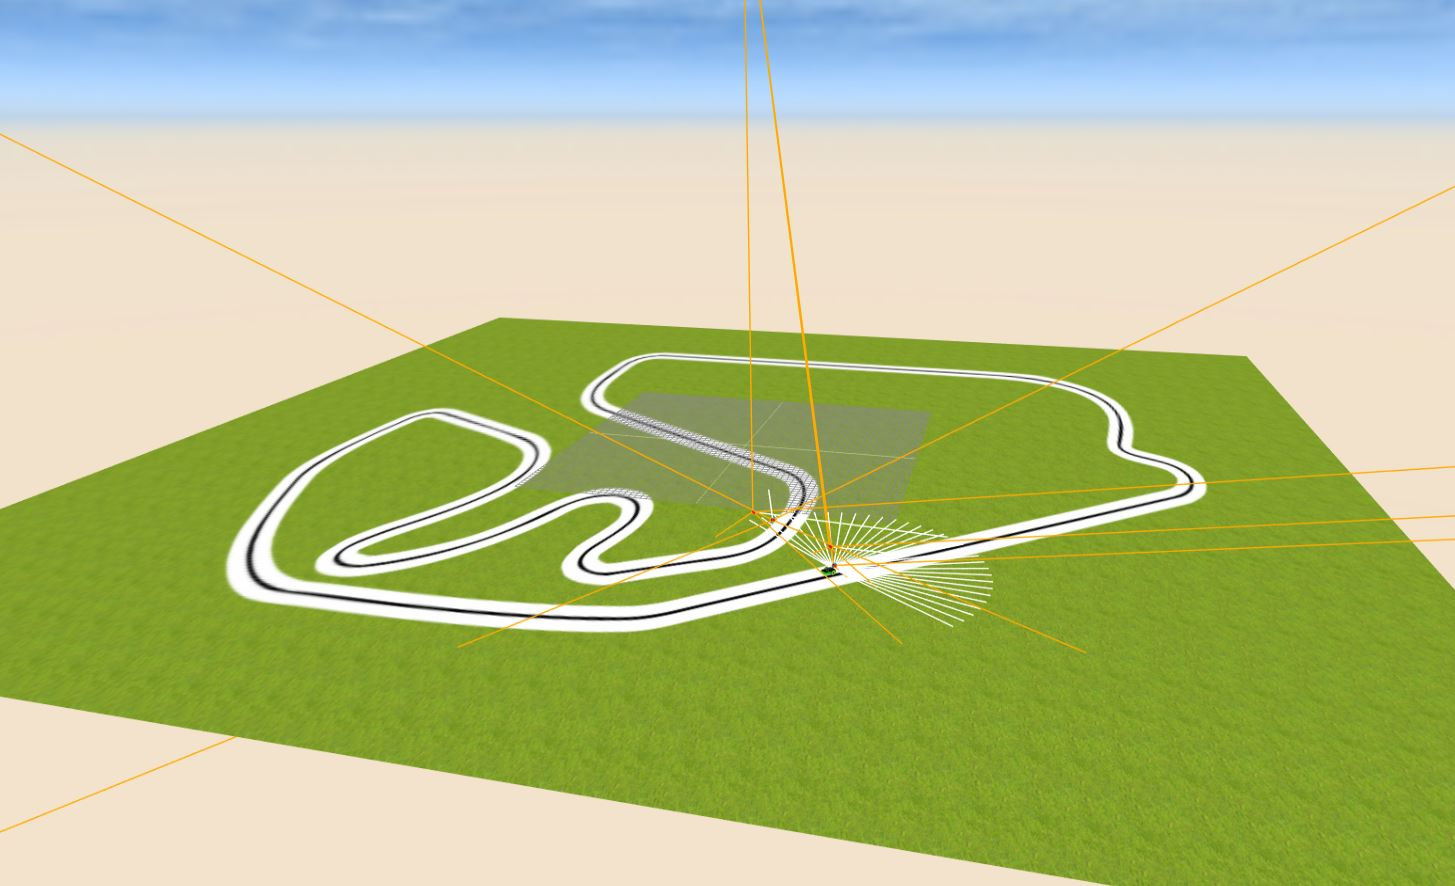
\includegraphics[scale=0.4]{img/siguelineas_ir.JPG}
    \caption{Escenario para el ejercicio \textit{piBot} sigue-líneas infrarrojo} \label{fig:siguelineasIR}
    \end{figure}
    
\subsection{Choca-gira}
Escenario creado en \textit{Blender} con un aspecto similar a su análogo en \textit{Python}. Para ello se han adaptado la mayor parte de las estructuras que dispone el escenario original para su integración en \textit{WebSim}. 

    \begin{figure}[H]
    \centering
    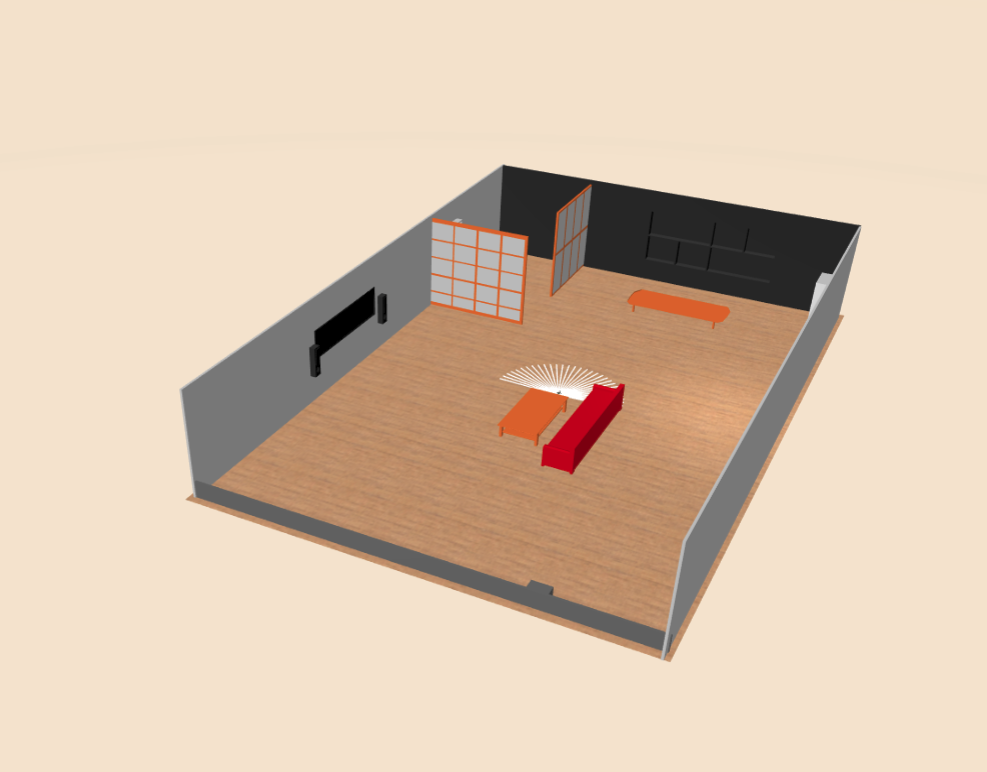
\includegraphics[scale=0.4]{img/bump&go.png}
    \caption{Escenario para el ejercicio choca-gira} \label{fig:chocagira}
    \end{figure}


\subsection{Sigue-pelota con piBot}
El escenario dispone de una pelota de color rojo a la que se le ha dado movimiento a través de primitivas de \textit{A-Frame}. En la figura \ref{fig:secuenciaPibot} se puede ver una secuencia con la animación de la pelota. 

\begin{figure}[htbp]
\begin{subfigure}[t]{0.2\textwidth}
    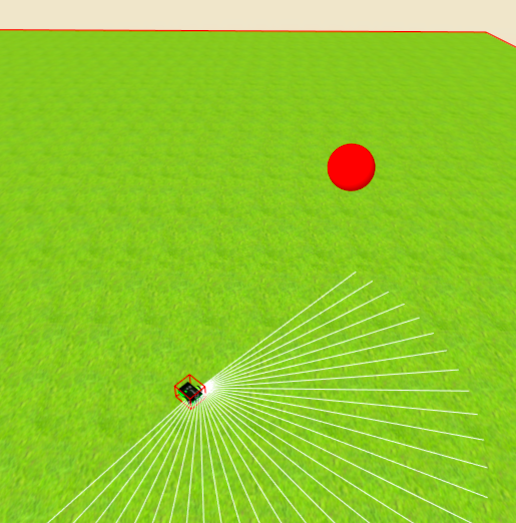
\includegraphics[width=3cm, height=3cm]{img/BallPibot1.png}
\label{fig:figure1_1}
\end{subfigure}\hfill
\begin{subfigure}[t]{0.2\textwidth}
  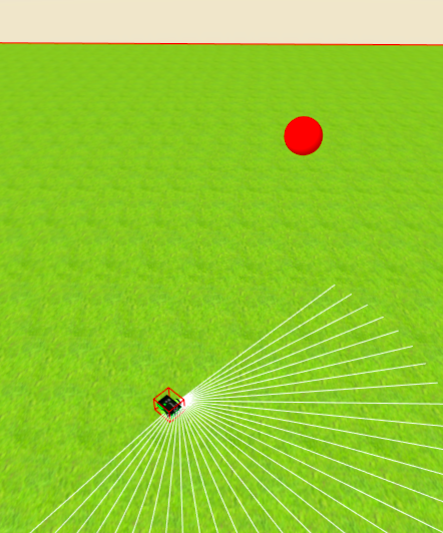
\includegraphics[width=3cm, height=3cm]{img/BallPibot2.png}
\label{fig:figure1_2}
\end{subfigure}\hfill
\begin{subfigure}[t]{0.2\textwidth}
    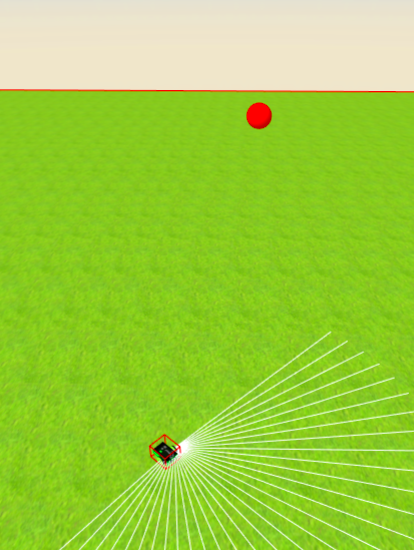
\includegraphics[width=3cm, height=3cm]{img/BallPibot3.png}
\label{fig:figure1_3}
\end{subfigure}

\begin{subfigure}[t]{0.2\textwidth}
    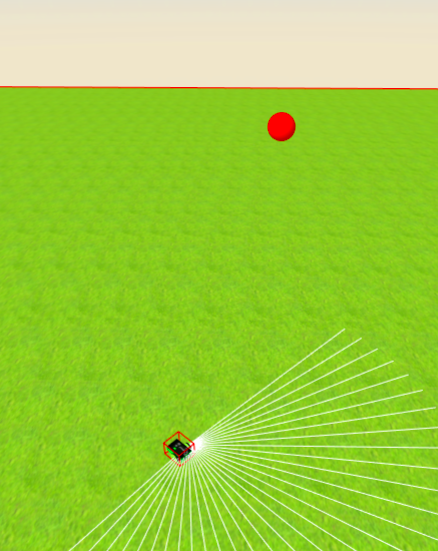
\includegraphics[width=3cm, height=3cm]{img/BallPibot4.png}
\label{fig:figure1_4}
\end{subfigure}\hfill
\begin{subfigure}[t]{0.2\textwidth}
    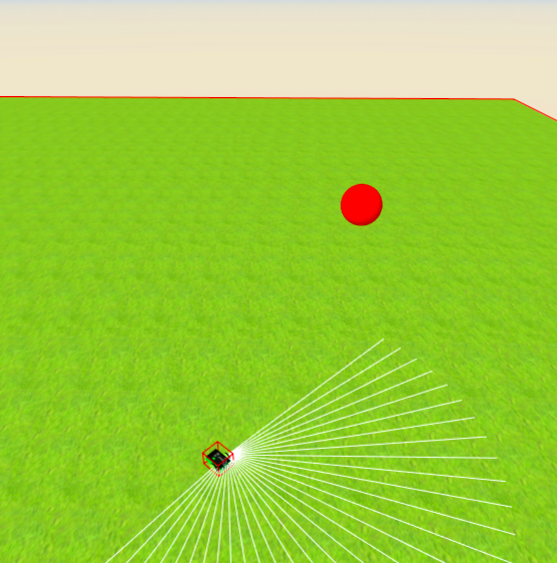
\includegraphics[width=3cm, height=3cm]{img/BallPibot5.png}
\label{fig:figure1_5}
\end{subfigure}\hfill
\begin{subfigure}[t]{0.2\textwidth}
    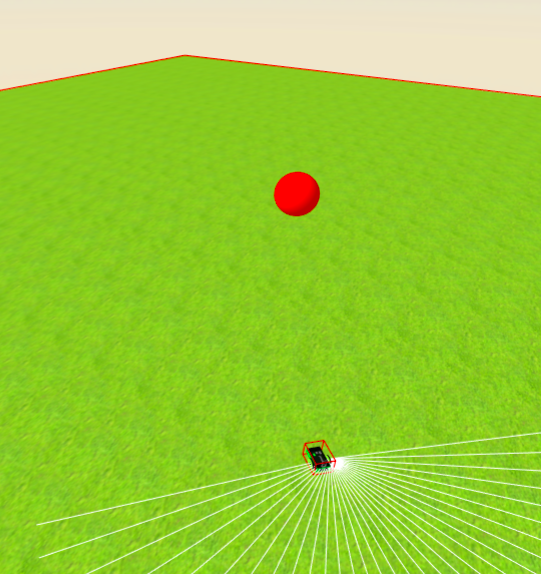
\includegraphics[width=3cm, height=3cm]{img/BallPibot6.png}
\label{fig:figure1_6}
\end{subfigure}

\begin{subfigure}[t]{0.2\textwidth}
    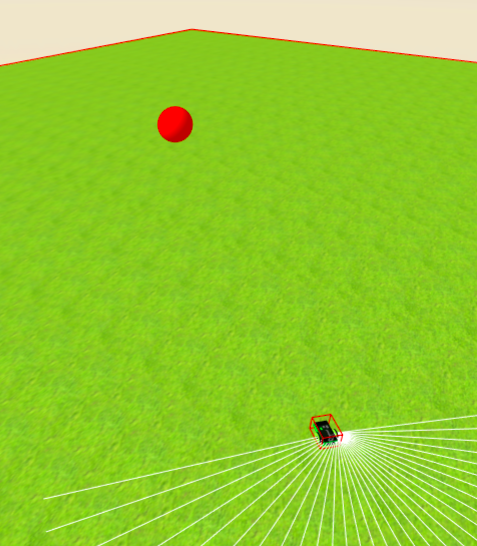
\includegraphics[width=3cm, height=3cm]{img/BallPibot7.png}
\label{fig:figure1_7}
\end{subfigure}\hfill
\begin{subfigure}[t]{0.2\textwidth}
    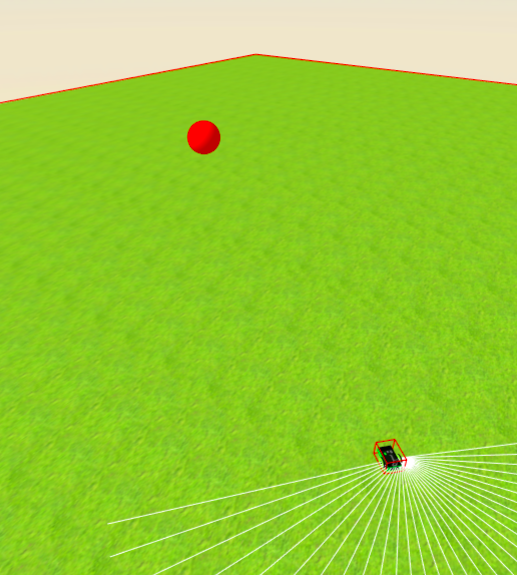
\includegraphics[width=3cm, height=3cm]{img/BallPibot8.png}
\label{fig:figure1_8}
\end{subfigure}\hfill
\begin{subfigure}[t]{0.2\textwidth}
    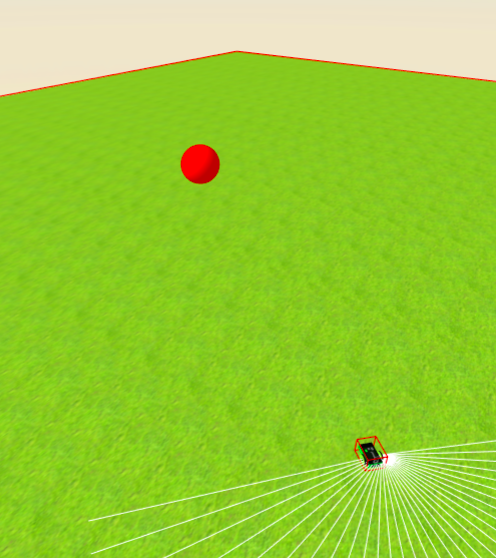
\includegraphics[width=3cm, height=3cm]{img/BallPibot9.png}
\label{fig:figure1_9}
\end{subfigure}
\caption{Secuencia de la animación de una pelota para el ejercicio piBot sigue-pelota}
\label{fig:secuenciaPibot}
\end{figure}

\subsection{Atraviesa-bosque}
Creado con primitivas de \textit{A-Frame}, el escenario tiene disposición de pasillo y diversos objetos en el camino para realizar un ejercicio que haga uso del sensor de ultrasonidos para evitar obstáculos.

    \begin{figure}[H]
    \centering
    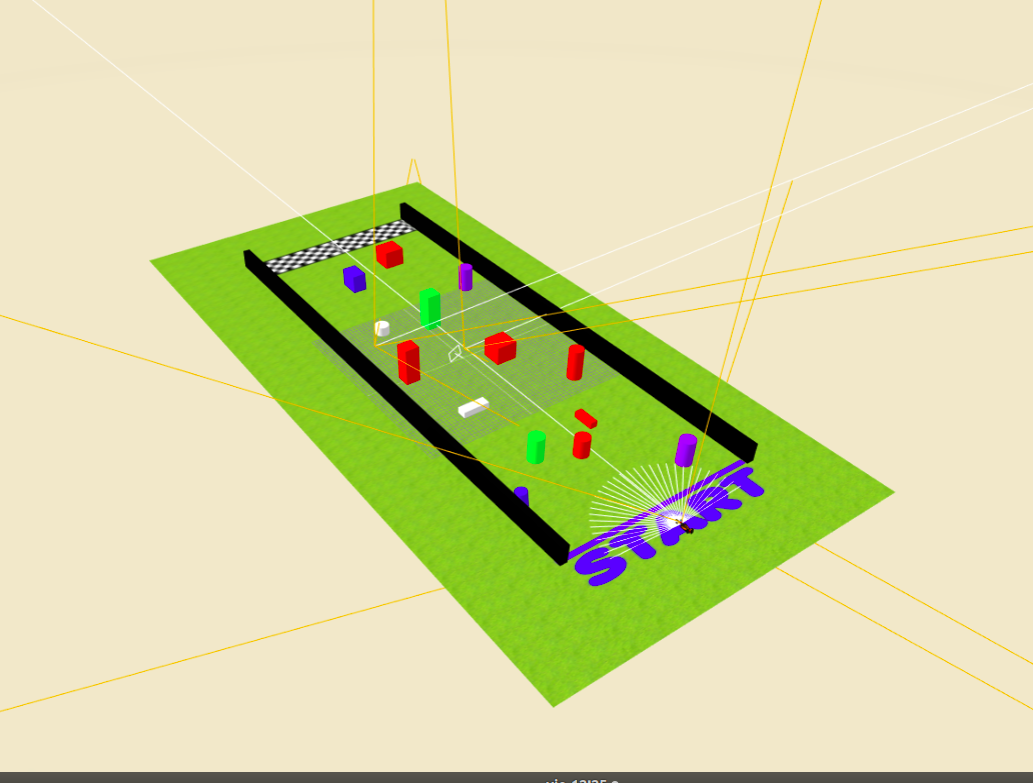
\includegraphics[scale=0.4]{img/atraviesabosque-indiv.png}
    \caption{Escenario para el ejercicio atraviesa bosque} 
    \label{fig:atraviesaBosqueind}
    \end{figure}
    
\subsection{Sigue-pelota con drone}
Realizado de forma similar al ejercicio con piBot, pero modificando la animación para que la pelota se mueva también en el eje Y. Se puede ver una secuencia de la animación en la figura \ref{fig:secuenciaDrone}.


\begin{figure}[htbp]
\begin{subfigure}[t]{0.2\textwidth}
    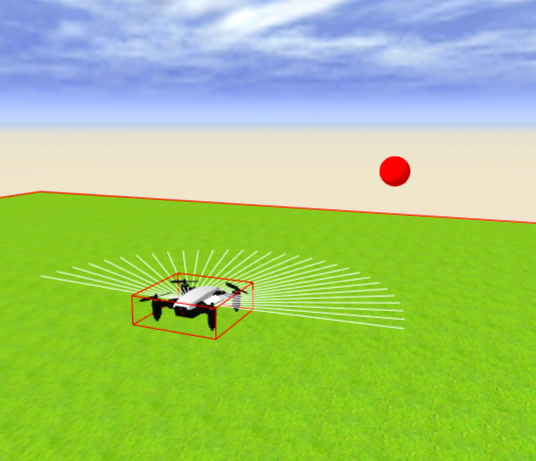
\includegraphics[width=3cm, height=3cm]{img/followBallTello1.png}
\label{fig:figure2_1}
\end{subfigure}\hfill
\begin{subfigure}[t]{0.2\textwidth}
  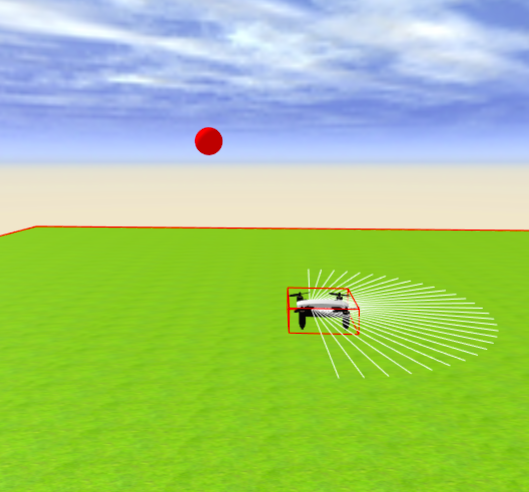
\includegraphics[width=3cm, height=3cm]{img/followBallTello2.png}
\label{fig:figure2_2}
\end{subfigure}\hfill
\begin{subfigure}[t]{0.2\textwidth}
    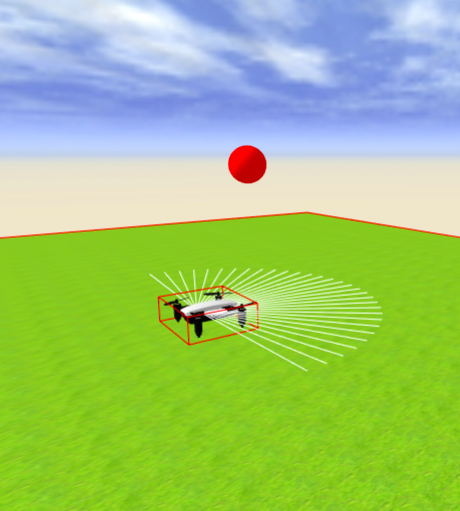
\includegraphics[width=3cm, height=3cm]{img/followBallTello3.png}
\label{fig:figure2_3}
\end{subfigure}

\begin{subfigure}[t]{0.2\textwidth}
    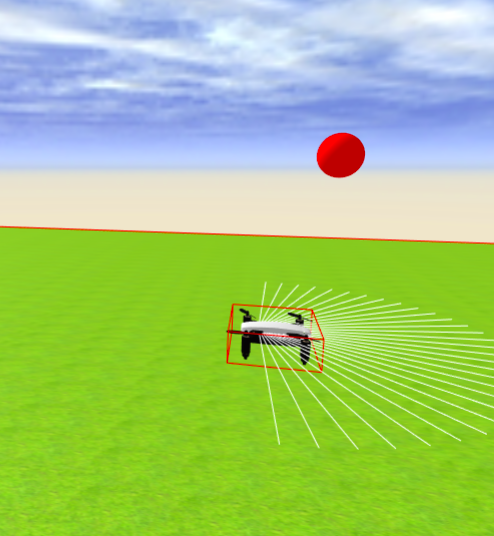
\includegraphics[width=3cm, height=3cm]{img/followBallTello4.png}
\label{fig:figure2_4}
\end{subfigure}\hfill
\begin{subfigure}[t]{0.2\textwidth}
    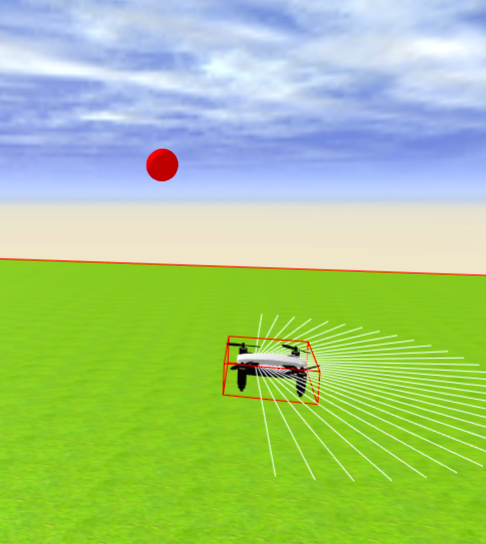
\includegraphics[width=3cm, height=3cm]{img/followBallTello5.png}
\label{fig:figure2_5}
\end{subfigure}\hfill
\begin{subfigure}[t]{0.2\textwidth}
    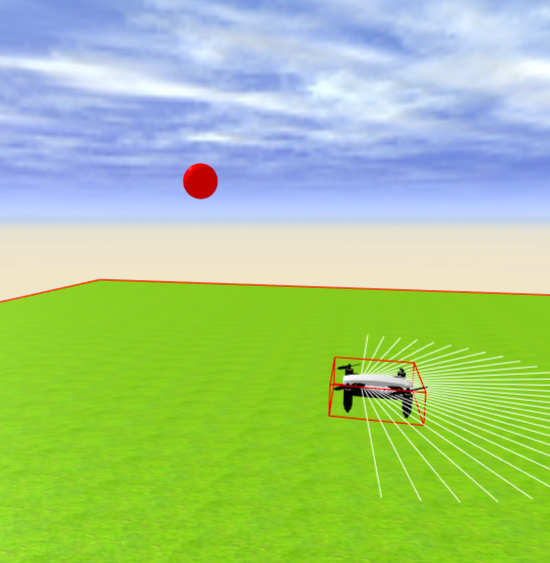
\includegraphics[width=3cm, height=3cm]{img/followBallTello6.png}
\label{fig:figure2_6}
\end{subfigure}

\begin{subfigure}[t]{0.2\textwidth}
    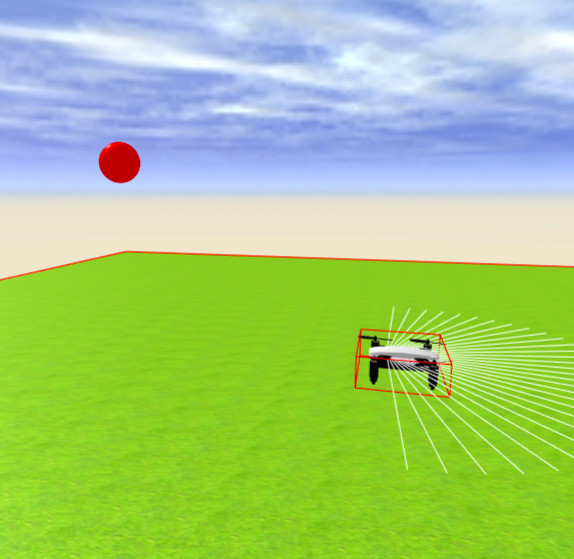
\includegraphics[width=3cm, height=3cm]{img/followBallTello7.png}
\label{fig:figure2_7}
\end{subfigure}\hfill
\begin{subfigure}[t]{0.2\textwidth}
    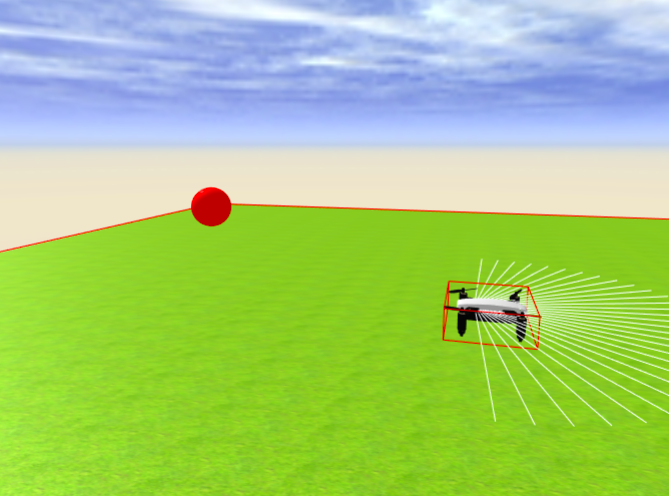
\includegraphics[width=3cm, height=3cm]{img/followBallTello8.png}
\label{fig:figure2_8}
\end{subfigure}\hfill
\begin{subfigure}[t]{0.2\textwidth}
    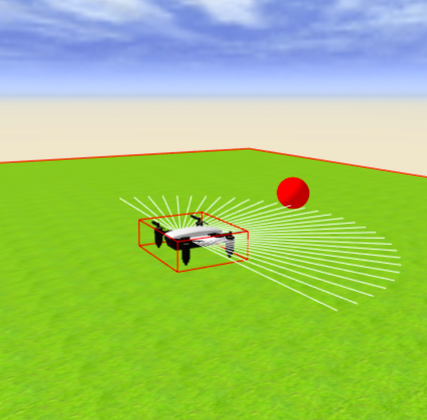
\includegraphics[width=3cm, height=3cm]{img/followBallTello9.png}
\label{fig:figure2_9}
\end{subfigure}

\begin{subfigure}[t]{0.2\textwidth}
    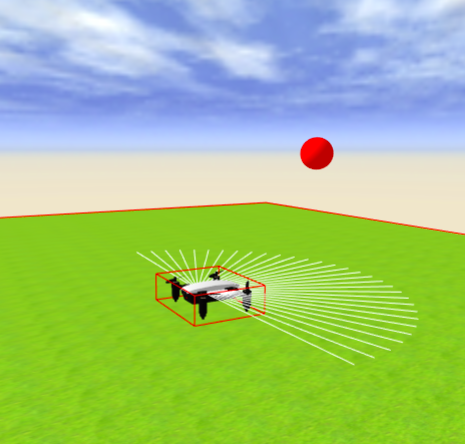
\includegraphics[width=3cm, height=3cm]{img/followBallTello10.png}
\label{fig:figure2_10}
\end{subfigure}\hfill
\begin{subfigure}[t]{0.2\textwidth}
    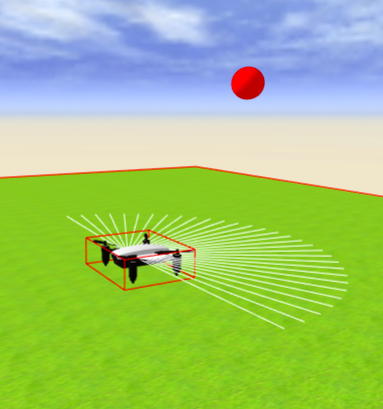
\includegraphics[width=3cm, height=3cm]{img/followBallTello11.png}
\label{fig:figure2_11}
\end{subfigure}\hfill
\begin{subfigure}[t]{0.2\textwidth}
    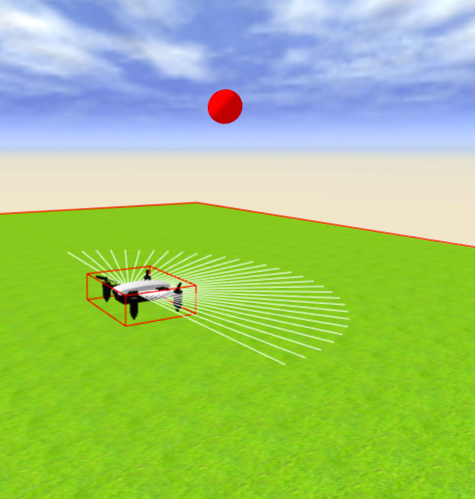
\includegraphics[width=3cm, height=3cm]{img/followBallTello12.png}
\label{fig:figure2_12}
\end{subfigure}
\caption{Secuencia de la animación de una pelota para el ejercicio \textit{drone} sigue-pelota}
\label{fig:secuenciaDrone}
\end{figure}

\subsection{Cuadrado con drone}

Escenario para facilitar el ejercicio ``cuadrado drone'' en el que hay que dibujar un cuadrado con el movimiento del \textit{drone}.
    
    \begin{figure}[H]
        \centering
        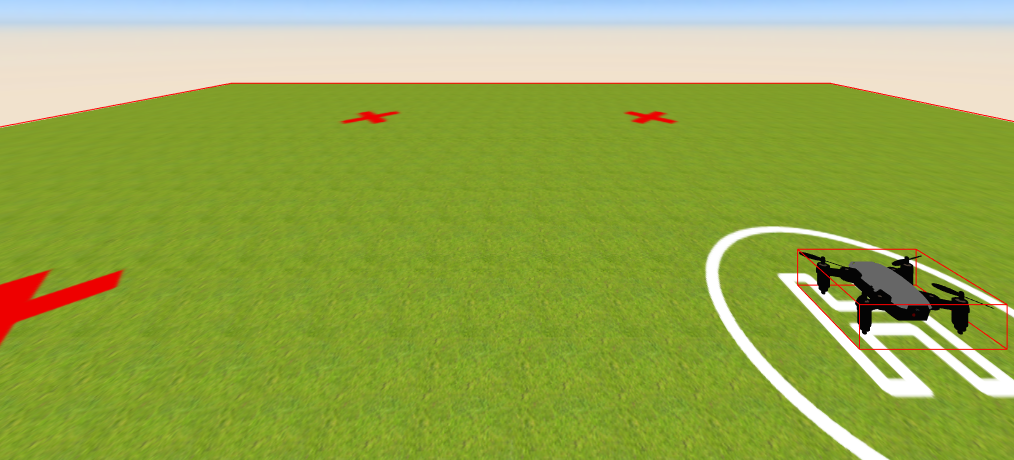
\includegraphics[scale=0.4]{img/cuadradoDrone.png}
        \caption{Escenario de WebSim para el ejercicio drone cuadrado} 
        \label{fig:droneCuadrado}
    \end{figure}
    
\subsection{Escenarios competitivos}

Se han realizado varios escenarios para realizar ejercicios competitivos:
\begin{itemize}
    \item Muros: prototipo creado para realizar pruebas comandando velocidades a los robots y comprobar el estado de sus sensores.
      
       \begin{figure}[H]
        \centering           
        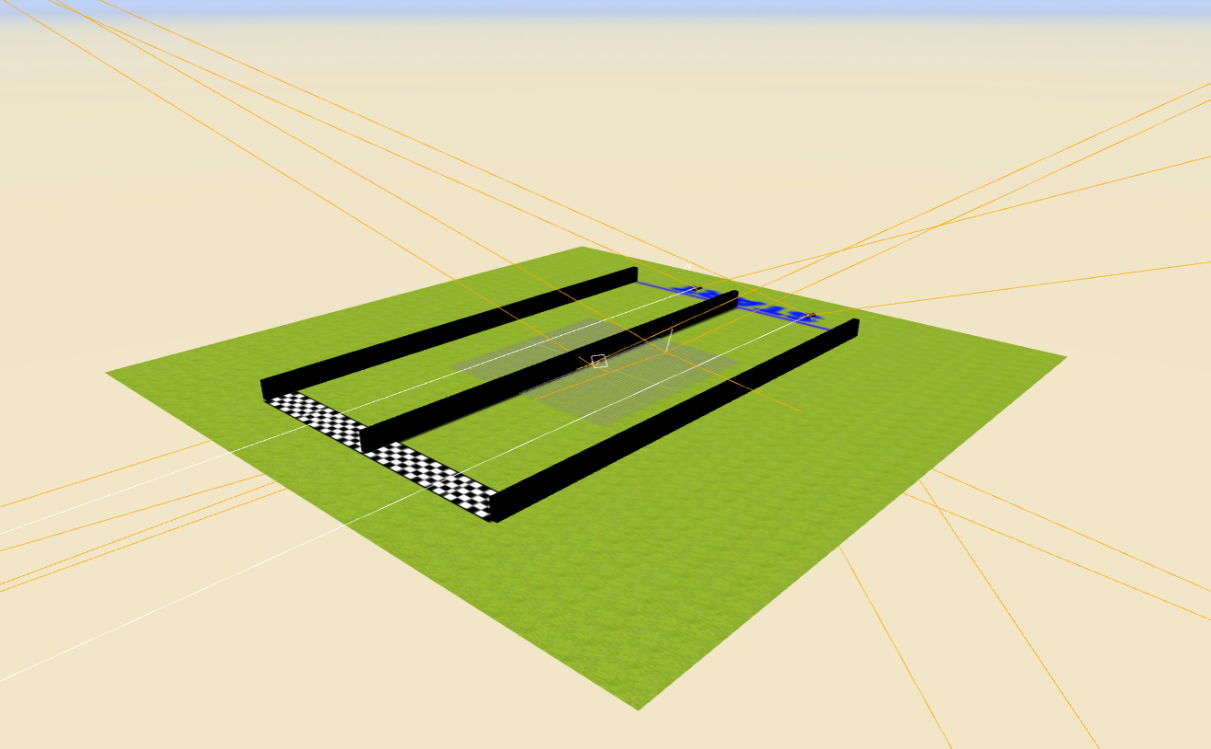
\includegraphics[scale=0.3]{img/ejercicio_muros.png}
        \caption{Prototipo ejercicio competitivo}
        \label{fig:ejercicio_muro}
    \end{figure}

    
    \item Atraviesa-bosque: ejercicio similar al escenario con un solo robot, pero en este caso se han creado dos pasillos con objetos para recorrerlos sin chocar con ninguno de los obstáculos. Se han añadido distintas primitivas de \textit{A-Frame} en la misma ubicación para los dos \textit{robots} para que el recorrido sea justo.
    
    \begin{figure}[H]
        \centering           
        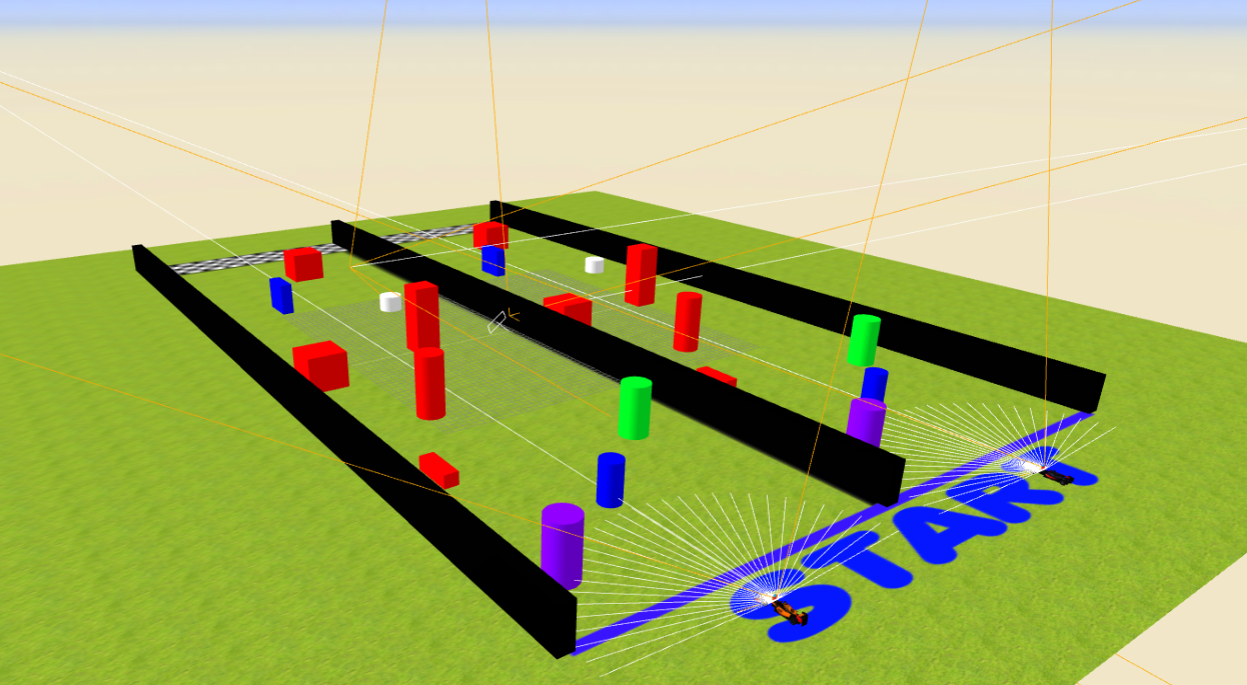
\includegraphics[scale=0.3]{img/ejercicio_atraviesabosque.png}
        \caption{Ejercicio atraviesa-bosque competitivo}
        \label{fig:atraviesabosque_escenario}
    \end{figure}
    
    \item Sigue-líneas: escenario con dos robots en el que tienen que seguir una linea de color blanco sobre fondo negro atravesando un puente en medio del circuito para que, de esta manera, ambos recorran la misma distancia.

    \begin{figure}[H]
        \centering            
        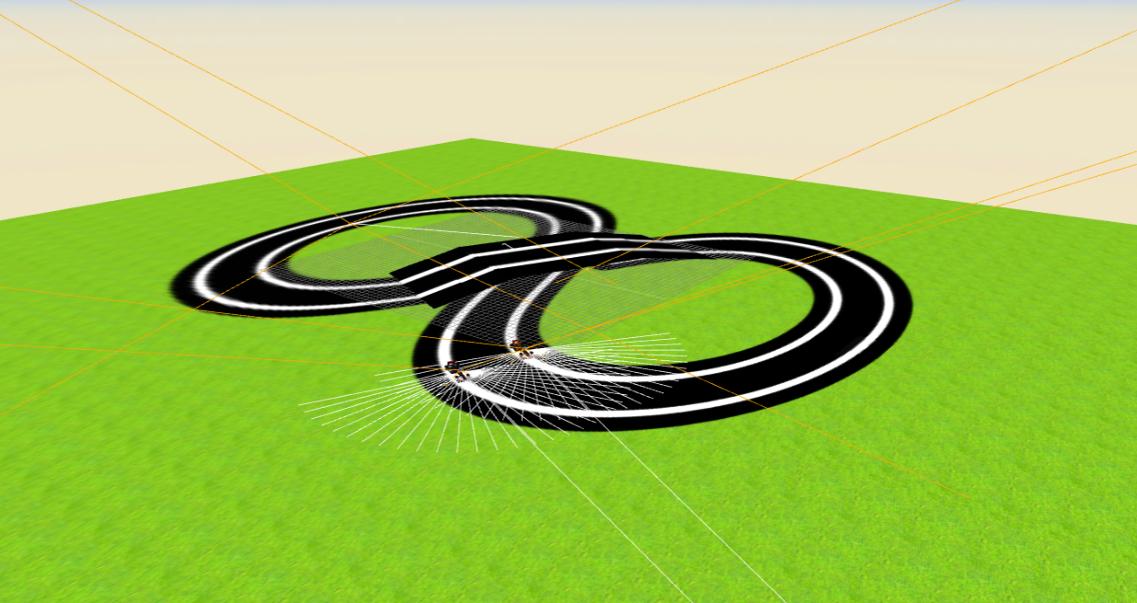
\includegraphics[scale=0.3]{img/ejercicio_siguelineas.png}
        \caption{Ejercicio sigue-líneas competitivo}
        \label{fig:siguelineas_competitivo}
    \end{figure}
\end{itemize}

Siendo el principal problema el puente creado para el ejercicio sigue-líneas. La solución definitiva ha sido creando primitivas de \textit{A-Frame} (\textit{a-plane}) de tal forma que simule un puente y pueda cruzarlo el coche. Se ha intentado realizar un modelo de puente en \textit{Blender}, pero el entorno no simulaba correctamente la malla de colisiones siendo imposible subir el puente porque el robot ``chocaba'' contra él. En la figura \ref{fig:prueba_puente} se puede ver el puente creado y la malla de colisión generada por \textit{A-Frame}.

    \begin{figure}[H]
        \centering            
        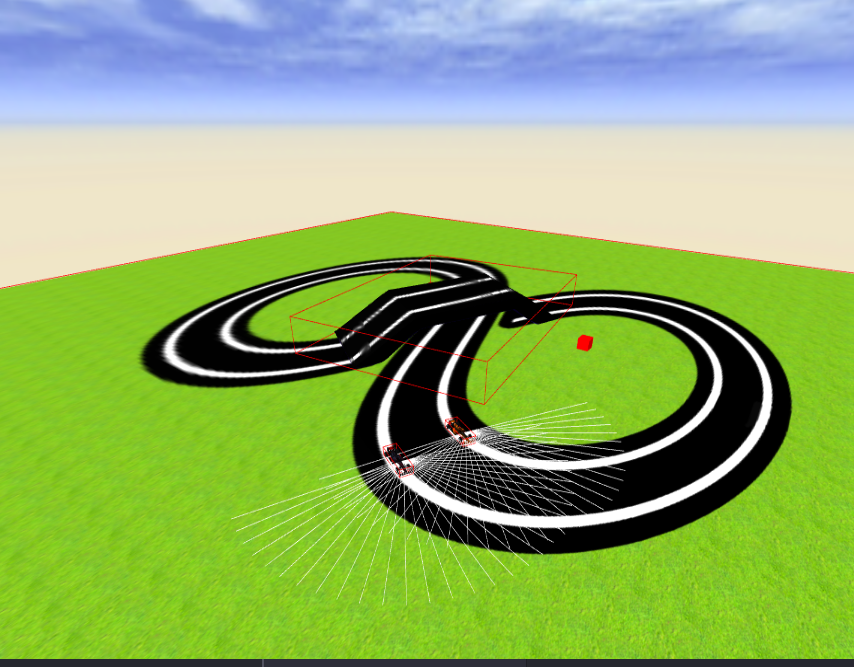
\includegraphics[scale=0.3]{img/prueba_puente.png}
        \caption{Prueba de puente creado en \textit{Blender}}
        \label{fig:prueba_puente}
    \end{figure}


\section{Teleoperadores}
Se han incorporado teleoperadores en \textit{WebSim} para poder controlar los robots sin necesidad de programarlos. De esta manera es posible saber el estado y valor de sus sensores de manera sencilla ayudando a los desarrolladores a buscar fallos en drivers o incorporar nuevos escenarios. 

\subsection{Ficheros de configuración}

Para incorporar estos teleoperadores ha sido necesario elaborar unos ficheros de configuración y así poder cambiar el escenario y el \textit{drone} cargado por \textit{A-Frame}. 

Estos archivos de configuración se han creado en \textit{JSON} (un formato de texto para representar datos estructurados en la sintaxis de objeto de \textit{JavaScript}) y se ha programado un \textit{script} para cargar cada fichero de configuración. Para ello se crea una variable en el \textit{index.html} del editor con la ruta en la que esté ubicado y el \textit{script} abre el fichero y recorre el \textit{JSON} para dar al escenario los valores establecidos. \newline

En los ficheros creados se pueden configurar aspectos como el modelo del robot cargado, su posición y rotación, la posición de la cámara a bordo del robot, el fichero del cielo y suelo que debe cargar o los elementos que queramos añadir en el escenario. \newline

\begin{lstlisting}[language=json, caption=Ejemplo de fichero de configuración]
  {
  "robot": {
    "model":"../assets/models/drone.gltf",
    "scale": "0.5 0.5 0.5",
    "position":"12 0 25",
    "rotation": "0 320 0"
  },
  "gravity": 0,
  "ground": "../assets/textures/escenarioLiso.png",
  "sky": "../assets/textures/sky.png",
  "secondaryCamera": "0 0 0",
  "cameraRobot":"0 0.03 -0.01",
  "objects":[{
      "type": "a-sphere",
      "position": "4 1 20",
      "color": "#FF0000"
      }
    ]
}
\end{lstlisting}

En este ejemplo se configura el escenario para que cargue el modelo del \textit{drone}, con el tamaño indicado en \textit{size}, la posición y rotación que aparece en \textit{position} y \textit{rotation}. En el valor \textit{gravity} se indica que el escenario no tenga gravedad, se carga la textura que posee el campo \textit{ground} como suelo del mundo y, por último, la posición de las cámaras es la ubicada en \textit{secondaryCamera} y \textit{cameraRobot}. Además, en \textit{objects} se pueden añadir todos los objetos deseados a la escena. En este ejemplo se añade una pelota de color rojo en la posición que aparece en \textit{position}.

\subsection{Teleoperadores}

Además de los modelos existentes del drone y \textit{piBot}, se han creado otros nuevos para extender las posibilidades de la plataforma y poder teleoperar todos ellos.
\begin{figure}[H]
    \centering            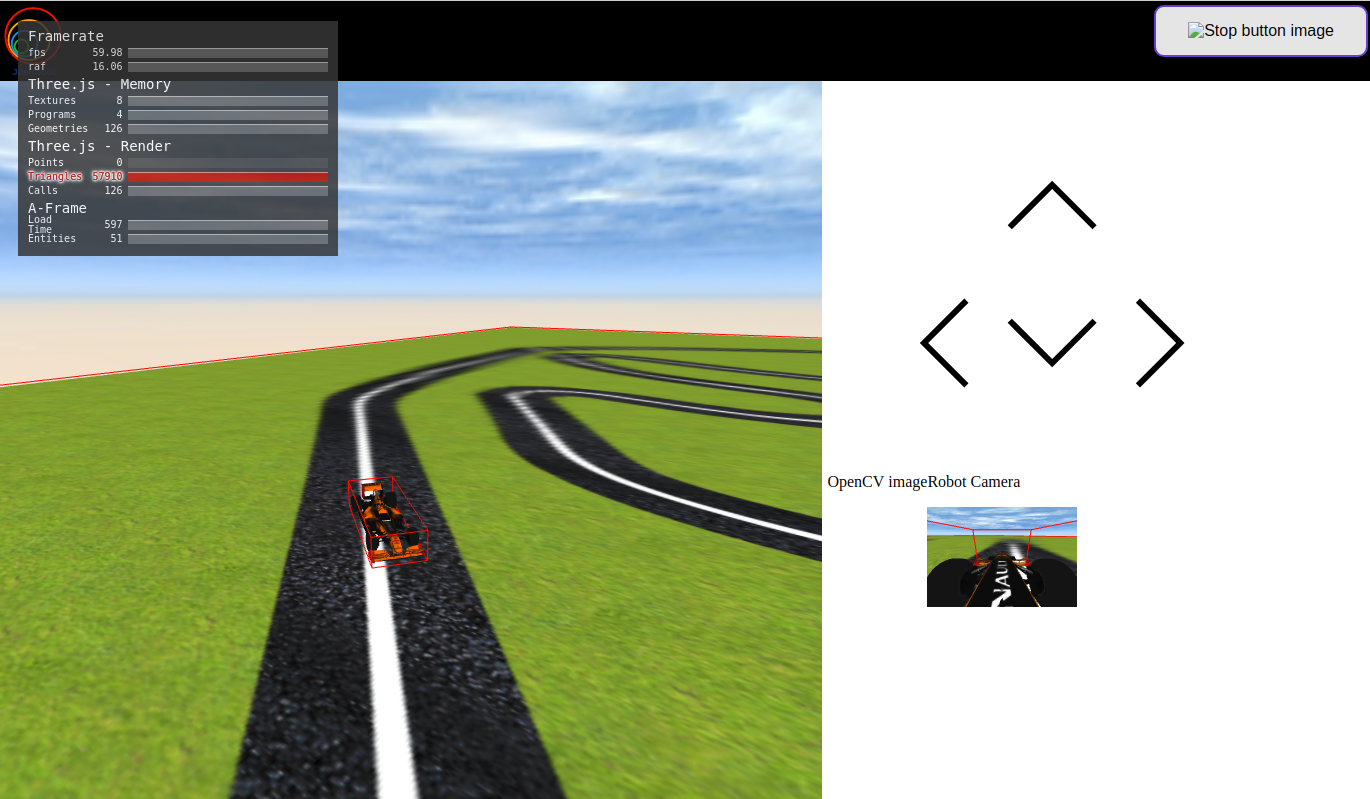
\includegraphics[scale=0.35]{img/f1_teleoperator.png}
    \caption{Teleoperador para el modelo del fórmula 1} \label{fig:f1_teleoperator}
\end{figure}
\begin{figure}[H]
    \centering            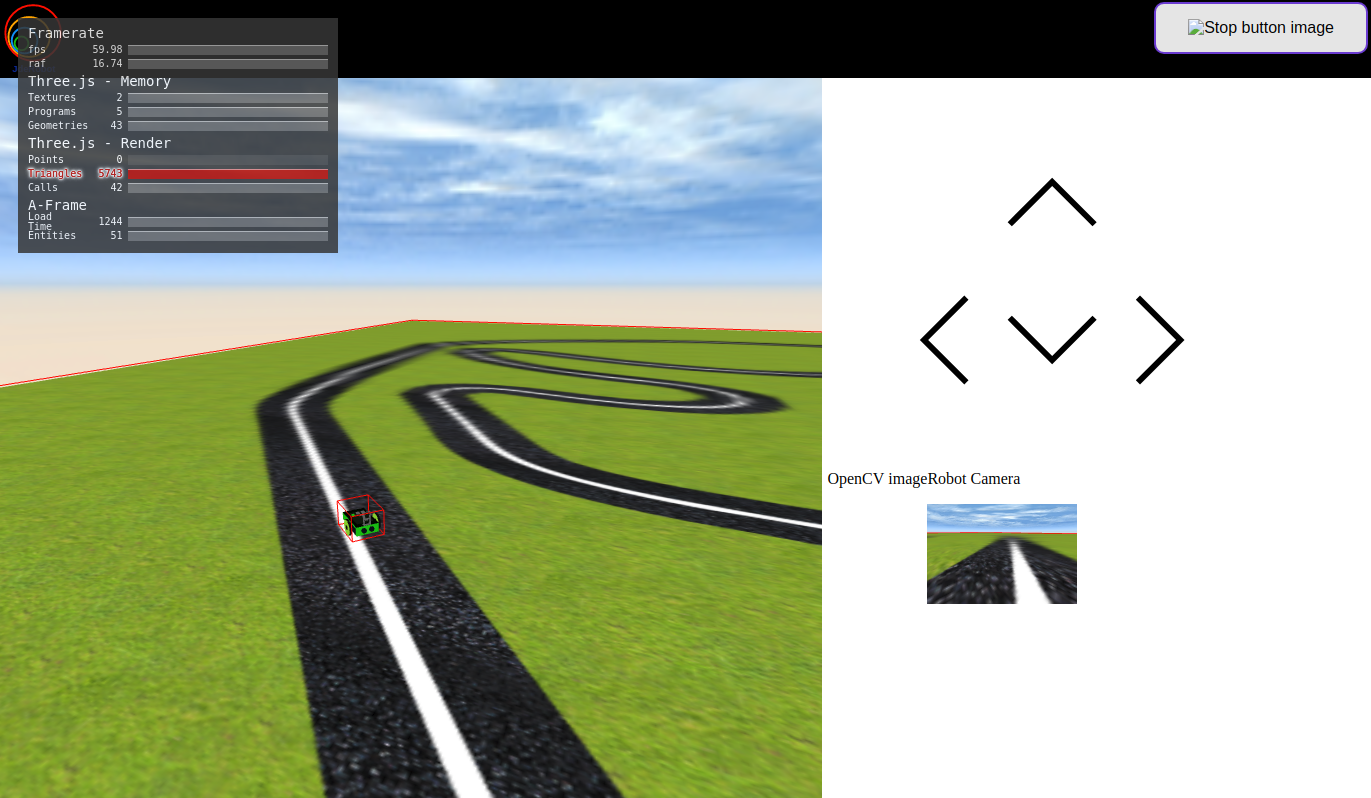
\includegraphics[scale=0.35]{img/pibot_teleoperator.png}
    \caption{Teleoperador para el modelo del piBot} \label{fig:piBot_teleoperator}
\end{figure}
  \begin{figure}[H]
    \centering
    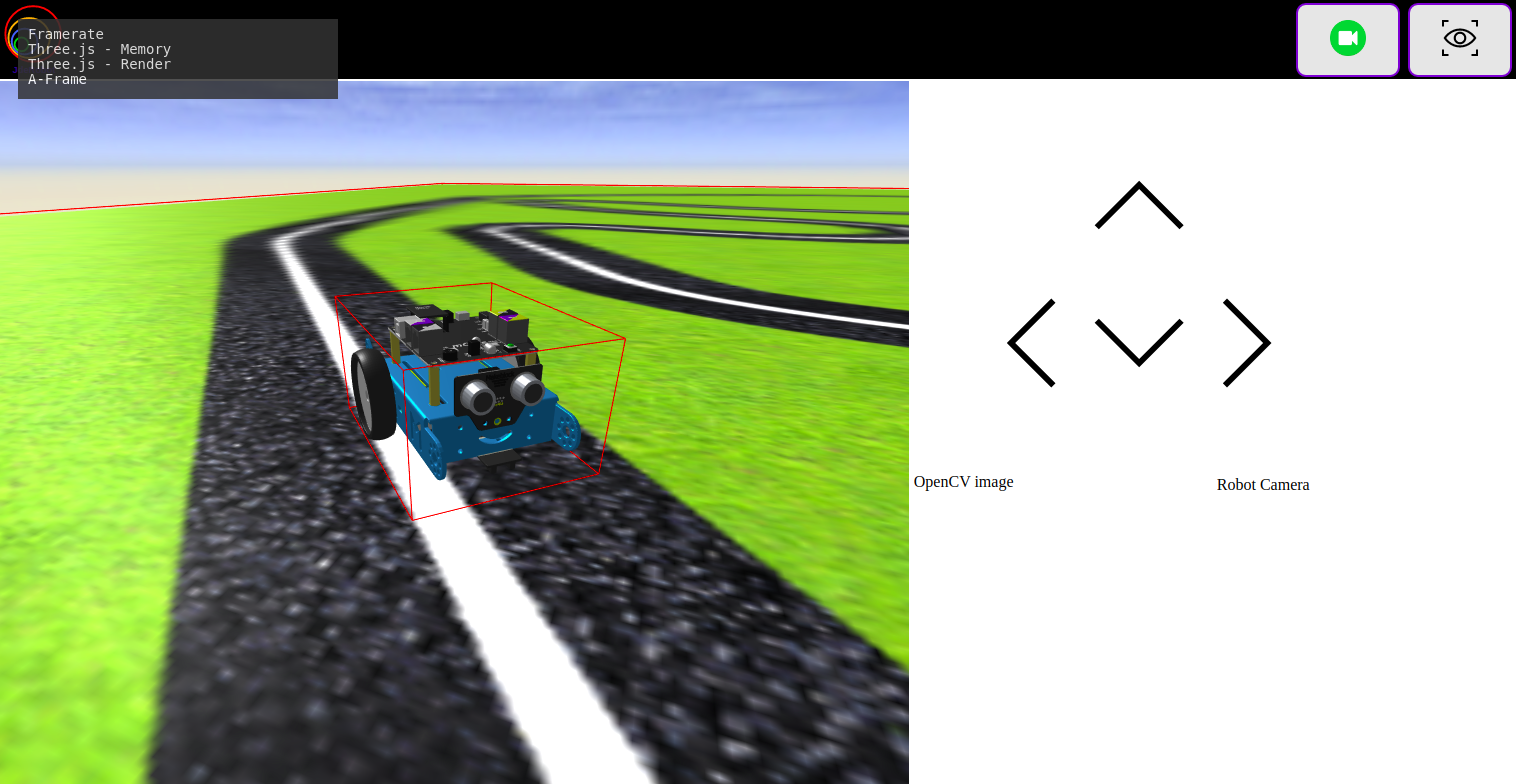
\includegraphics[scale=0.3]{img/mBot_teleoperator.png}
    \caption{Teleoperador para el modelo del mBot} \label{fig:mBot_teleoperator}
\end{figure}
\begin{figure}[H]
    \centering
    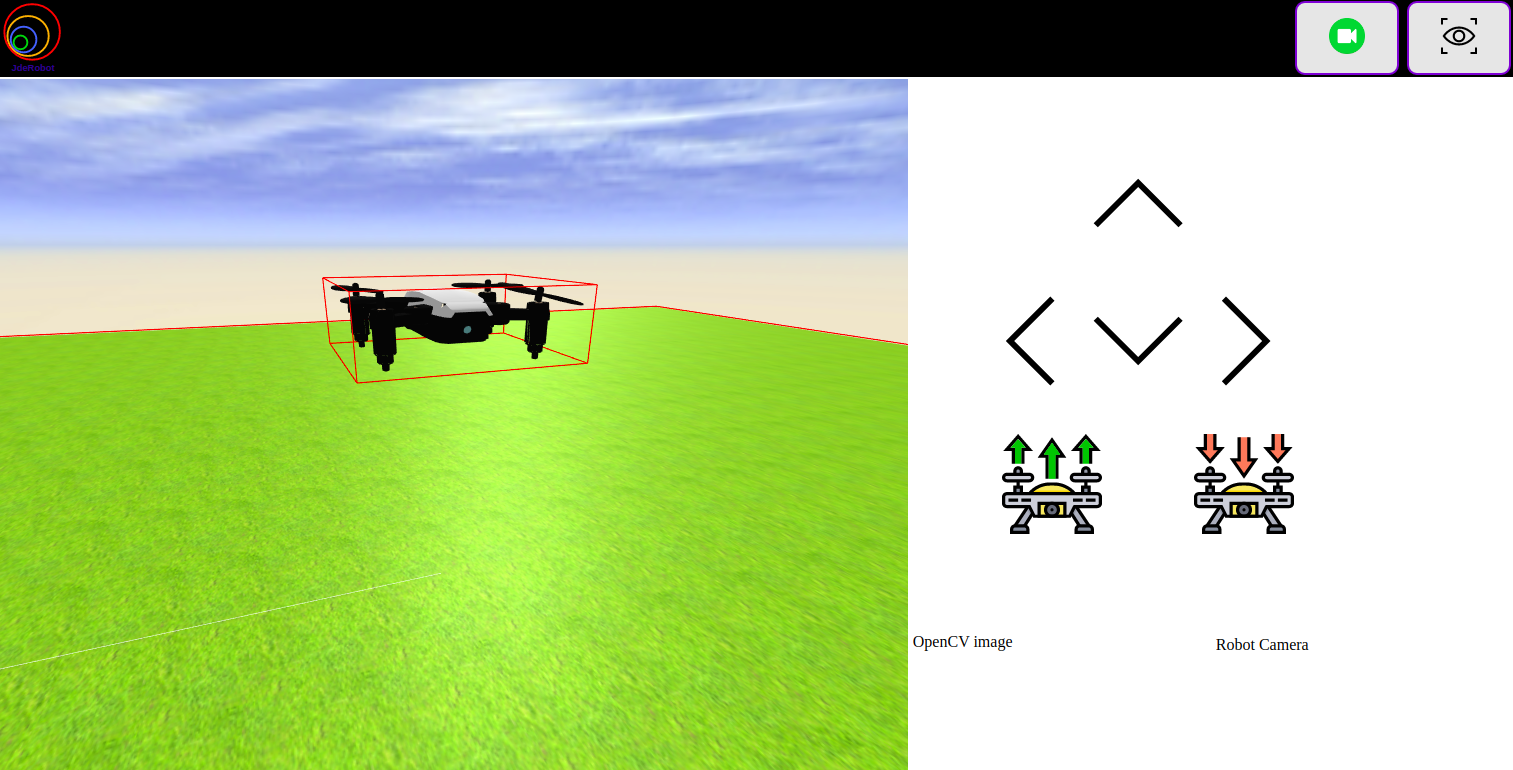
\includegraphics[scale=0.3]{img/drone_teleoperator.png}
    \caption{Teleoperador para el modelo del drone} \label{fig:drone_teleoperator}
\end{figure}
    
Pudiendo controlar todos ellos con los botones que aparecen en la imagen o bien a través del teclado. 
Además, se ha creado una página principal para poder acceder a todos ellos a través de una interfaz gráfica: 

 \begin{figure}[H]
    \centering
    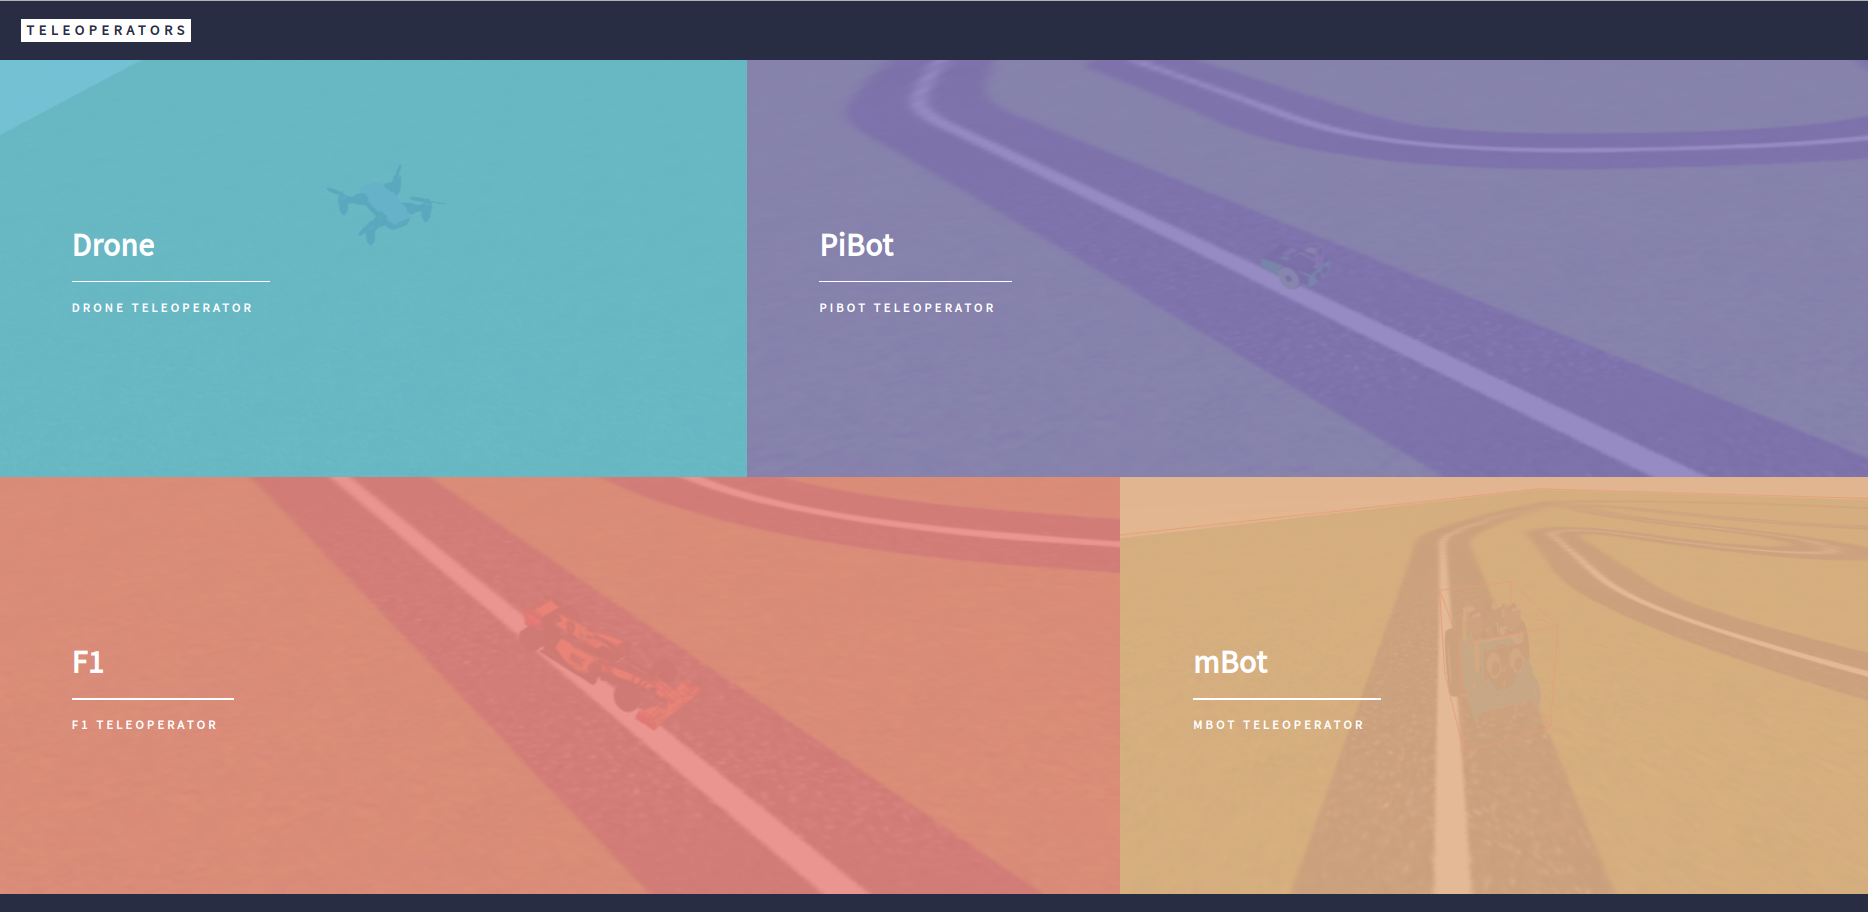
\includegraphics[scale=0.25]{img/teleoperators.png}
    \caption{Interfaz que permite acceder a cada uno de los teleoperadores} \label{fig:teleoperators}
\end{figure}

\section{Ejercicios competitivos}

Uno de los objetivos de este proyecto era añadir ejercicios competitivos. Se hace especial mención a ellos debido a que son completamente diferentes al resto de los ya creados. Este tipo de ejercicios aumenta el valor de la plataforma ya que da la posibilidad de programar dos robots en el mismo escenario, pudiendo entender la programación como un juego en el que se premia al que aporte la mejor solución.

%  Para dar soporte a este tipo de ejercicios se ha realizado una refactorización de \textit{WebSim}, actualizando así la aplicación a la versión \textit{WebSim 2.0}. En esta versión se separan los hilos de \textit{HAL API}, simulador y editor dando la posibilidad de crear más de un robot en la misma escena, cambiar el código del robot en la simulación o incluso parar la simulación y reanudarla después con un código distinto. \newline

En este tipo de ejercicios hay dos robots en una misma escena donde cada uno de ellos se puede programar con un código distinto. Para facilitar la integración con el resto de la plataforma se han incorporado dos aplicaciones más a \textit{WebSim}: ejercicios competitivos en \textit{Scratch} y ejercicios competitivos en \textit{JavaScript}. 


Se ha comenzado creando la aplicación llamada \textit{competitive-JavaScript} debido a la facilidad para probar código y hacer pruebas en el entorno. Para ello se ha cambiado la interfaz del editor, añadiendo botones para cada uno de los robots (figura \ref{fig:javascript_competitivo}) y añadir funcionalidad a cada botón para guardar el código de cada robot o mostrar el código en caso de tener uno guardado.

    \begin{figure}[h]
        \centering            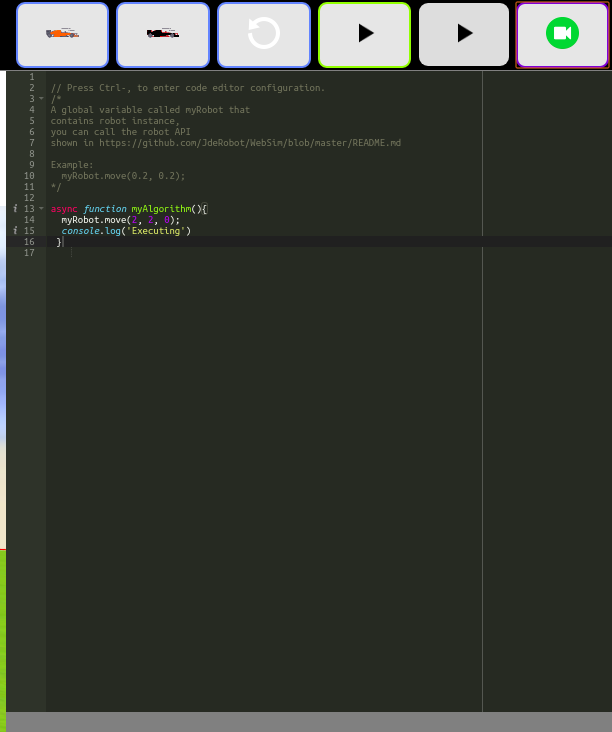
\includegraphics[scale=0.30]{img/competitiveEditorJavascript.png}
        \caption{Editor de \textit{JavaScript} para ejercicios competitivos}
        \label{fig:javascript_competitivo}
    \end{figure}

La aplicación \textit{competitive-Scratch} se ha realizado de la misma manera, con la diferencia de que, en este caso, es necesario guardar el código de los bloques en \textit{XML} y su traducción en \textit{JavaScript}. Para realizarlo de forma limpia se ha creado un objeto que contiene un \textit{boolean} y dos cadenas de texto. En el \textit{boolean} se indica el código de qué \textit{robot} se está editando, en una cadena de texto se guarda el código \textit{XML} y en la otra su traducción en \textit{JavaScript}. Se puede ver la interfaz de este editor en la figura \ref{fig:scratch_competitivo}.

    \begin{figure}[h]
        \centering            
        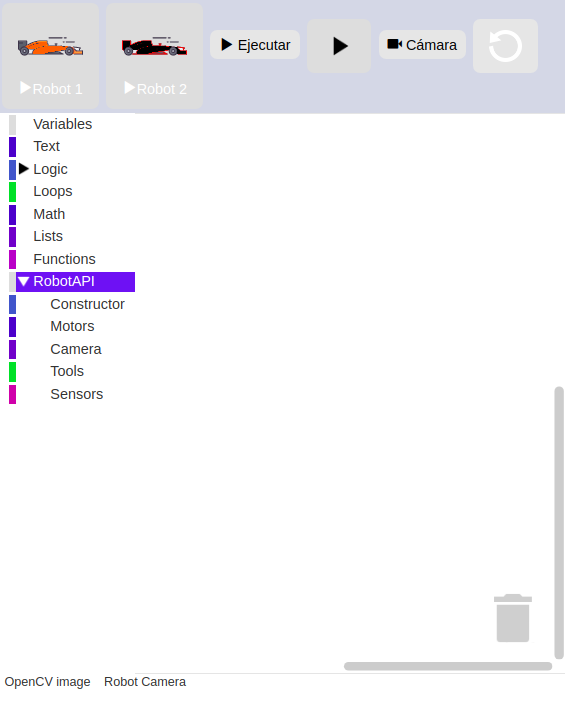
\includegraphics[scale=0.30]{img/competitivoEditorScratch.png}
        \caption{Editor de \textit{Scratch} para ejercicios competitivos}
        \label{fig:scratch_competitivo}
    \end{figure}
    
Para puntuar el comportamiento de los robots de manera justa, se han incluido en estos ejercicios evaluadores automáticos. Van a tener diferentes comportamientos en cada ejercicio, por lo que se han desarrollado de tal forma que se pueda cargar cargar un evaluador distinto para cada uno o, incluso, no cargar ninguno. \newline

Para su implementación se ha creado la función \textit{runEvaluator}, que acepta como parámetro un \textit{array} con los identificadores de los robots y el archivo del evaluador deseado. Este fichero se recoge como variable en el \textit{index.html} del editor correspondiente (de forma similar a los archivos de configuración). 
Para llamar a \textit{runEvaluator} se comprueba que se haya pasado un fichero en el \textit{index.html} y, si eso ocurre, se realiza un \textit{require} de ese fichero y se ejecuta la función principal del evaluador, \textit{evaluator.main()}. Esta se encarga de llamar a las funciones necesarias para que el evaluador sea completo: crea la interfaz gráfica y la lógica necesaria para su correcto funcionamiento.

A continuación se explican los ejercicios y evaluadores para cada uno de ellos. 

\subsection{Atraviesa-bosque competitivo}

Para este ejercicio se usa el escenario de la imagen \ref{fig:atraviesabosque_escenario}. Se ha creado un evaluador en el que se crea una barra de progreso para cada robot y un cronómetro. Cuando se empiezan a mover los robots la barra de progreso se va completando y el cronómetro se inicia, para comprobar el porcentaje completado solo hay que obtener la posición del robot y compararla con el punto de llegada.

\begin{figure}[H]
\centering           
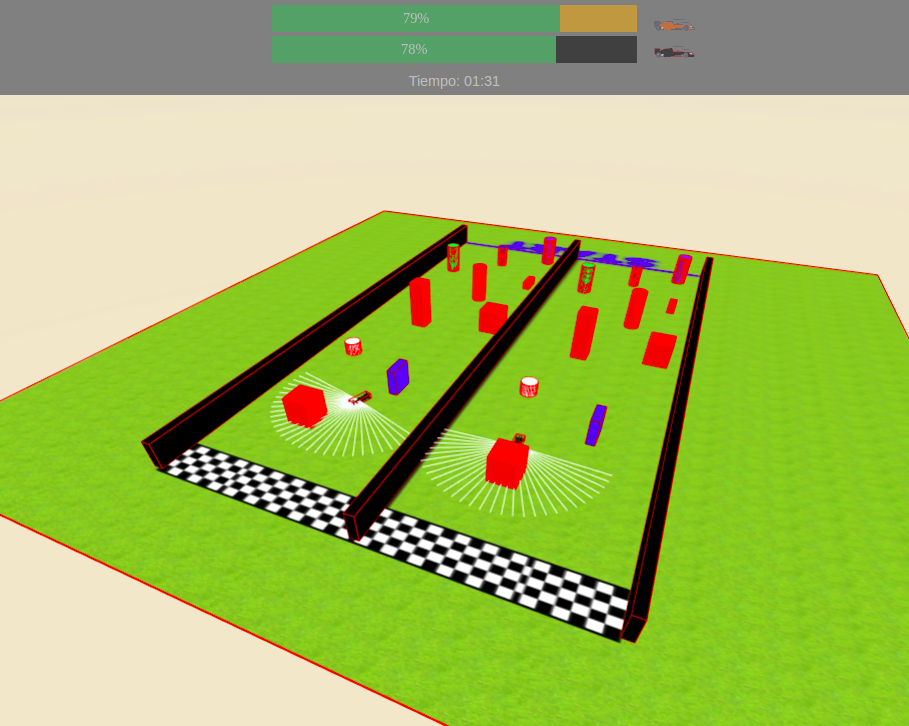
\includegraphics[scale=0.3]{img/evaluador_forest.png}
\caption{Evaluador para el ejercicio atraviesa-bosque}
\label{fig:evaluador_bosque}
\end{figure}


\subsection{Sigue-líneas competitivo}

Para este ejercicio se usa el escenario de la figura \ref{fig:siguelineas_competitivo} y su evaluador es similar al de atraviesa-bosque, con la diferencia de que es necesario guardar en todo momento la posición y distancia recorrida por cada robot para calcular el porcentaje del circuito completado.


\begin{figure}[H]
    \centering           
    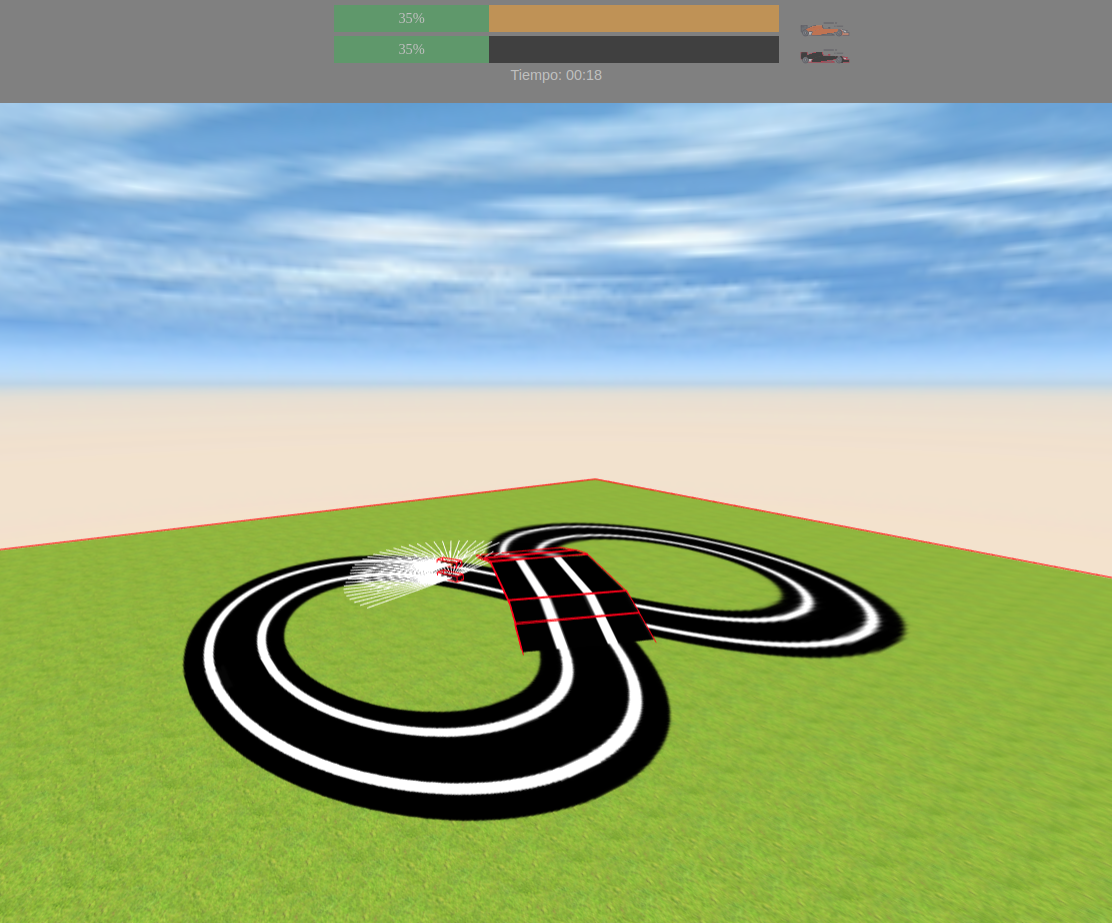
\includegraphics[scale=0.25]{img/evaluator_follow_line.png}
    \caption{Evaluador sigue-líneas}
    \label{fig:evaluador_siguelineas}
\end{figure}

\subsection{Gato-ratón}

Con la nueva estructura de \textit{WebSim} se permite realizar el ejercicio gato-ratón con \textit{drones}. Se trata de otro tipo en el que no se compite con dos códigos programados por distintos usuarios, si no que un \textit{drone} ya está programado y el usuario solo tiene que desarrollar su solución para que el \textit{robot} no se aleje del objetivo. Para ello ha sido necesario crear un modelo al que se le ha pintado de color rojo para que sea más sencillo su filtrado. Se puede ver el nuevo modelo de \textit{drone} en la figura \ref{fig:drone_rojo}.


Para el evaluador de este ejercicio se crea un gráfico con ayuda de una librería externa de \textit{JavaScript} (\textit{JavaScript Graphics Library}\footnote{\url{http://www.jsgl.org/}}) que muestra la distancia entre \textit{drones} y el tiempo que lleva de ejecución. Se puede ver este evaluador en la figura \ref{fig:evaluador_gato_raton}.
  
    \begin{figure}[h]
    \centering           
    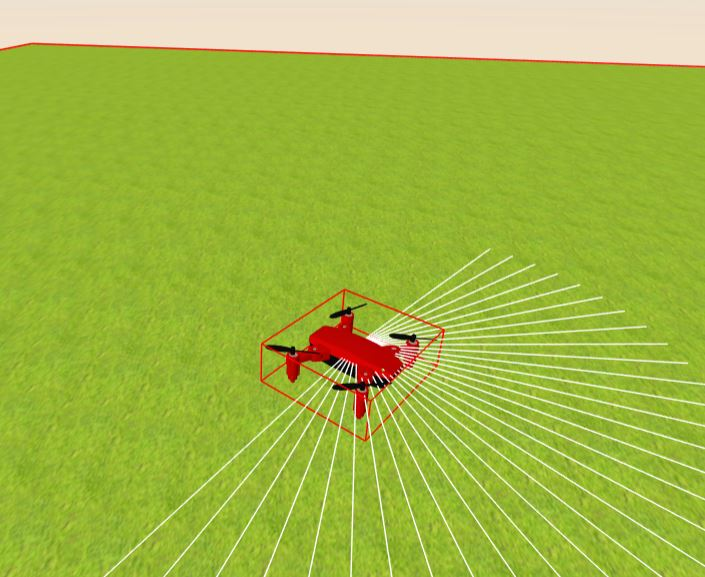
\includegraphics[scale=0.5]{img/red_drone.jpg}
    \caption{Nuevo modelo de drone para ejercicio gato-ratón}
    \label{fig:drone_rojo}
    
\end{figure}
\begin{figure}[h]
\centering           
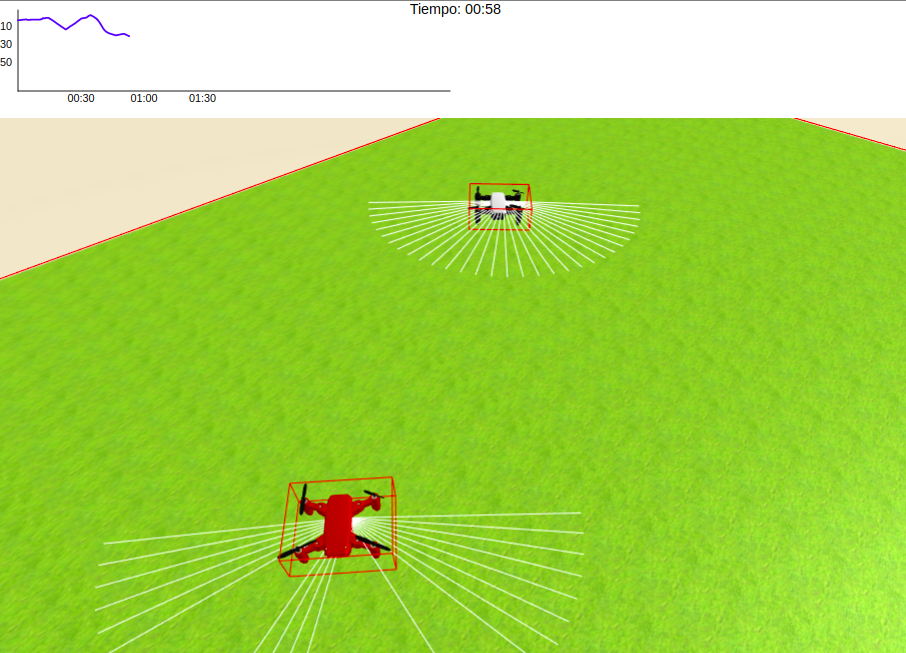
\includegraphics[scale=0.3]{img/evaluador_drone.png}
\caption{Evaluador para ejercicio gato-ratón}
\label{fig:evaluador_gato_raton}
\end{figure}
